\documentclass[arial,11pt]{article}
\usepackage[dvips]{graphicx}
%\documentclass[11pt]{nih}
\usepackage{amssymb}
%\usepackage{graphicx}
%\usepackage{longtable}
\usepackage{epsfig}
%\usepackage{overcite}
\usepackage[usenames]{color}
%\usepackage{multibbl}
\usepackage[colorlinks=true,linkcolor=black]{hyperref}

\renewcommand{\rmdefault}{phv} % Arial
\renewcommand{\sfdefault}{phv} % Arial
\renewcommand{\thesection}{\Alph{section}}
\pagestyle{empty}

%\usepackage{times}
\usepackage{geometry}
%\geometry{tmargin=1in,bmargin=1.0in,lmargin=1in,rmargin=1in}
\geometry{tmargin=0.95in,bmargin=0.95in,lmargin=0.95in,rmargin=0.95in}
%\linespread{0.95} \interfootnotelinepenalty=10000

%%%%% editing helpers
\newcommand{\NeedRevision}[1]{\textcolor{red}{#1}}

\begin{document}

%\newbibliography{snets}

\begin{center}
{\Large {\bf Technology and Research Development Project 3: \\
Spectral archives and spectral networks}}
\end{center}

\section{Specific aims}

When CCMS started there was no software for clustering millions (let alone, billions) of spectra and the concept of spectral networks (that enabled antibody and antibiotics sequencing) was just published and still in the early proof-of-concept stage. This is unfortunate since spectral archives are a prerequisite for the automatic large-scale construction of spectral libraries and to fully realize the potential utility of mass spectrometry data repositories. CCMS developed the first spectral archives and spectral networks software and applied it in many joint projects with experimental researchers. While we demonstrated how to construct spectral archives with a billion spectra~\cite{frank11}, the problem of clustering {\em all} publicly available spectra remains open - a key goal of the world-wide mass-spectrometry repository MassIVE proposed by CCMS in 2012 and covered here and in TRD8.

The spectral networks paradigm pioneered at CCMS differs from the mainstream database search paradigm in three fundamental ways. First, spectral networks are based on matching spectra against other spectra instead of against protein sequences. Second, spectral networks find spectra from related peptides (e.g., modified/unmodified or overlapping-sequence variants) even before considering their possible identifications. Third, spectral networks determine consensus identifications for {\em sets} of spectra from related peptides instead of separately attempting to identify one spectrum at a time. After substantial algorithmic developments, spectral networks have now delivered the longest ($\approx 10\times$ longer than single-spectrum sequencing) and most accurate ($\approx 98\%$ sequencing accuracy) {\em de novo} sequences to date~\cite{bandeira08,guthals12metasps}, confirmed the new route for discovery of unexpected post-translational modifications and highly-modified peptides~\cite{gonzalez10,yang11,guthals12specnets}, enabled the automated sequencing of non-linear (e.g., cyclic) non-ribosomal peptides~\cite{bandeira08recomb,ng09} and are now defining a novel molecular spectral networks approach for mapping the entire molecular output of any biological system suitable for analysis with tandem mass spectrometry~\cite{watrous12,moree12}.

%     \begin{itemize}
%        \item Library matching is the current "gold standard"
%        \item Clusters and networks reveal "known unknowns"
%        \item Networks reveal related peptides
%        \item Networks enable multiple-alignment-based consensus interpretations - best de novo sequencing ever
%     \end{itemize}
%
%
%     \begin{itemize}
%        \item SL-GF for library search and construction of networks
%        \item Spectrum alignment models based on expected variations
%        \item Spectral probability models for spectral networks propagations
%        \item Extend consensus interpretations from de novo to DB IDs
%        \item Extend consensus interpretations from single-spectrum matching to matching sample spectral-networks to network libraries
%     \end{itemize}

In the new cycle CCMS will integrate spectral archives and spectral networks algorithms by focusing on the following specific aims, which relate to one another as illustrated in Figure~\ref{trd.snets.fig.aims}:

%development of new spectral matching and spectral alignment algorithms based on models of differential peptide fragmentation between spectra of related peptides (in one or more fragmentation modes) and will integrate these with generating functions (similarly to the MS-GF approach introduced by CCMS) to derive new models of statistical significance for spectrum/spectrum matches. The resulting identifications and spectral networks will then be used to a) propagate identifications from identified to unidentified spectra and b) directly identify spectral networks by extending our de novo sequencing algorithms to $i$) database search (as in our previous extensions of MS-Dictionary to MS-GF+) and $ii$) spectral library search (by extending our M-SPLIT library search algorithms).

\begin{itemize}
    \item {\bf Aim 1: Prediction and matching of tandem mass spectra using spectral projections.} A core operation in spectral library search is to assess whether two spectra are generated from related peptides \-- a task that would reduce to simple spectrum matching if we could predict spectra for any peptide of interest. In difference from current methods designed to predict spectra directly from peptide sequences~\cite{paizs05,zhang05,zhang10}, we propose a new {\em spectral projection} approach for predicting spectra from other spectra (of related peptides).
%spectral prediction approach based on {\em spectral projection} models of {\em differential} peptide fragmentation between spectra of related peptides. We further propose methods for more efficient spectral matching to accelerate clustering, library search and construction of spectral networks.
%     \begin{itemize}
%        \item SL-GF for library search and construction of networks; Extend SLGF to put more weight on peaks distinguishing between close runner-up IDs (e.g., site-localization)
%        \item Projections / spectrum alignment models based on expected variations
%        \item Joint PRM/Projection scoring models
%        \item Extend to trillions of spectra: use tiered networks 1) propagate using same-sample nets after matching to 1) libraries, 2) unmod DB, 3) simple-mods DB, 4) restricted archive
%        \item Extend to trillions of spectra: using sequence tags to filter pairs
%     \end{itemize}

    \item {\bf Aim 2: Construction of spectral networks using spectral dictionaries.} We propose a new Spectral Library Generating Function (SL-GF) approach (similar to the MS-GF~\cite{kim08} approach introduced by CCMS) to derive new models of statistical significance for Spectrum-Spectrum Matches (used to define edges in spectral networks). In addition, we extend the CCMS-proposed concept of spectral dictionaries~\cite{kim09msdict,jeong11} to {\em network dictionaries} of all peptides that match {\em all} spectra in a spectral network in a statistically significant way.
% (used to define connected components in spectral networks).
%     \begin{itemize}
%        \item Network dictionaries
%        \item Network projections? Capturing the concept of "allowable" variation within a network?
%        \item Scale network construction to Billions (maybe Trillion) spectra: hashing, tags - VERY limited pairwise alignments
%        \item Networks archive for trillions of spectra: tiered networks archive with a record of similar spectra from distinct / unknown peptides
%     \end{itemize}

    \item {\bf Aim 3: Peptide identification in spectral networks via spectral library and database search.} In cases when spectral networks aggregate both identified and unidentified spectra, we will use the structure of the network and a customized Target-Decoy Approach to propagate identifications from identified to unidentified spectra at a fixed false discovery rate (FDR). We further propose a new approach to identify spectral networks by database search of consensus spectra derived from spectral networks.
% and propose a new way to use sample-specific PTM frequencies to adjust peptide-spectrum match scores.

%        and b) directly identify spectral networks by extending our de novo sequencing algorithms to $i$) database search (as in CCMS's previous application of spectral dictionaries to MS-GFDB~\cite{kim10cidetd}) and $ii$) spectral library search (by extending our M-SPLIT~\cite{wang10} library search algorithms).
%     \begin{itemize}
%        \item Spectral probability models for spectral networks propagations
%        \item Extend consensus interpretations from de novo to DB IDs
%        \item Extend consensus interpretations from single-spectrum matching to matching sample spectral-networks to network libraries
%     \end{itemize}

    \item {\bf Aim 4: Molecular spectral networks for spectra from any type of molecules.} We generalize the concept of spectral networks using structure-independent algorithms to construct spectral networks for spectra from any type of molecules suitable for analysis with tandem mass spectrometry.
This extends the original concept of spectral networks (aimed at peptides) to diverse  set of compounds.
%In difference from the peptide-specific or instrument-specific methods in aims 1-3, this aim proposes graph-based methods to $i)$ filter network edges %and $ii)$ define connected components in molecular spectral networks.
\end{itemize}

\begin{figure*}[!htb]
\centering
%\scalebox{1.0}{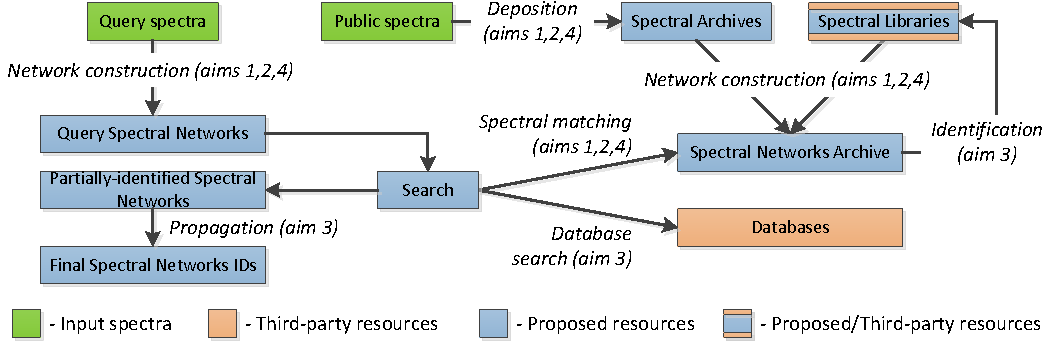
\includegraphics{figures/overview.eps}}
\scalebox{1.0}{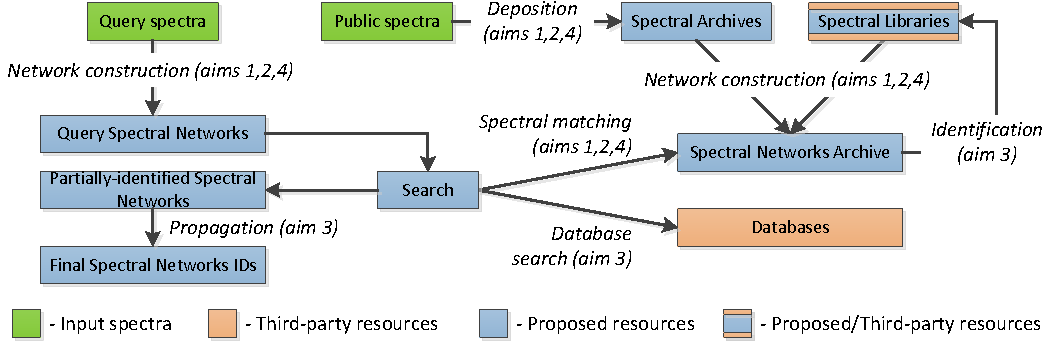
\includegraphics[width=\textwidth]{figures/overview.pdf}}

\caption{\footnotesize{\bf Contextualized Specific Aims.} {\em Spectral Networks} connect spectra of related peptides; {\em Spectral Libraries} are collections of identified reference spectra; {\em Spectral Archives} are collections of unidentified spectra clustered into unique reference spectra from all public spectra. The goal of this TRD is to develop the algorithms required to progress towards identification of all query spectra by $1)$ using correlations between query spectra to build spectral networks which are then identified by matching against $2a)$ spectral libraries or $2b)$ sequence databases and $3)$ by further propagating such identifications to unidentified query spectra using query spectral networks. Finally, $4)$ matching to the spectral archive reveals whether the remaining query spectra are ``novel'' or have been previously observed in other conditions/species in publicly released data.}
\label{trd.snets.fig.aims}
\end{figure*}

%*******************************************
\section{Significance}
%*******************************************

% Extended introduction - how spectral networks are different and why they are relevant

The dominant paradigm for high-throughput protein identification is based on trypsin digestion of extracted proteins to produce peptides followed by tandem mass spectrometry to generate single-peptide spectra that are then matched one spectrum at a time against protein databases~\cite{eng94,perkins99,craig04,tanner05} to obtain peptide and protein identifications. This database search paradigm has been the basis of nearly all large-scale proteomics studies to date despite its typical low spectrum identification rate of only 15-30\%. Nevertheless, this is endured because enzymatic digestion generates multiple peptides per protein and, in the extreme, only one peptide needs to be identified to call a protein identification (the main goal in most proteomics experiments). The downside of this low identification rate is that it consistently leads to missing information on non-tryptic peptides
%(e.g., protein N-term)
and yields low protein sequence coverage, thus substantially limiting the chances of detecting alternative splicing or
%to identify and localize post-translational modifications (
PTMs. In fact, the limitations of PTM search are so dire that most labs still only allow for 4-6 PTMs per search (about half or which due to sample handling procedures) even though more than 500 PTMs are listed in UniMOD. Metaproteomics analysis of environmental samples from host-pathogen interactions~\cite{zheng11} and microbial communities (as in the Human Microbiome Project) further requires the ability to search mass spectrometry data against very large databases and, in many cases, against six-frame translations of poorly-annotated genomes or even draft assemblies (as proposed in TRD1). This enormous growth in the size of the sequences database and the need to allow for polymorphisms and/or unexpected PTMs results in a combined search space so large that 90-95\% of all spectra are  discarded as unidentified. This computational bottleneck severely limits proteomics analysis of the role of microbiomes in health and disease~\cite{pflughoeft11}.

Peptidomics, defined as the study of endogenous peptides, is an abundant source of drug candidates derived from neuropeptides~\cite{robertson11}, toxins~\cite{king11} and non-linear cyclic peptides~\cite{colgrave10}. Endogenous peptides are also valuable as therapeutic targets~\cite{jaggi11} (neuropeptides) and antigenic peptides are key in immunotherapeutic strategies~\cite{depontieu09} (MHC class-I/II peptides). Despite its critical importance, peptidomics research continues to suffer from the inadequate reutilization of computational tools primarily developed for proteomics since (a) endogenous peptides are not suitable for enzymatic digestion (as it eliminates the active peptide form), (b) tend to be modified with unexpected PTMs, (c) often contain sequence polymorphisms and (d) generally lack the ``MS-friendly'' features of trypsin-digested peptides. As such, each endogenous peptide must be identified ``on its own'' (not being able to benefit from multiple peptides per protein as in proteomics) and new identification algorithms are needed to handle non-tryptic peptides of atypical lengths~\cite{jaggi11} (e.g., $\leq$6 AA or $\geq$35 AA) containing unexpected PTMs, sequence polymorphisms~\cite{klug09,colgrave10} and often featuring non-linear structures~\cite{king11,colgrave10}.

One possible way to improve identification of endogenous peptide is to search their spectra against spectral libraries.
 Spectral libraries are collections of peptide spectra whose identifications were validated by statistical methods~\cite{keller02,elias07} and were often also manually validated by mass spectrometry experts. The growing availability of these large collections of MS/MS spectra has reignited the development of alternative peptide identification approaches based on spectral matching~\cite{craig06,frewen06,lam07,wang10} algorithms. The potential of spectral libraries to improve identification of endogenous peptides is well illustrated by the CCMS-developed NeuroPedia~\cite{kim11neuropedia} spectral library of neuropeptide spectra. By capitalizing on previously-observed features in library spectra (e.g., actual fragment intensities, neutral losses from fragments, and various uncommon or even unknown fragments), NeuroPedia was shown to improve neuropeptide identification by up to tenfold at the same false discovery rate~\cite{lam10}.

The concept of spectral libraries (based on storing identified spectra) was recently extended by CCMS to spectral {\em archives} including ``interesting'' non-identified spectra~\cite{frank11}, which are constructed by clustering all observed spectra. In MS/MS analysis, it is common for peptides to get selected for fragmentation more than once~\cite{tabb03a}. When mass spectra are collected from many sources (as in MassIVE), such redundancies can add up to many thousands of spectra from the same peptides. Instead of repeating the identification process for each spectrum, it can be beneficial to perform the search only once using a representative consensus spectrum per peptide and later apply the results to all clustered spectra~\cite{tabb03a,beer04,tabb05}. By analyzing only representative spectra (one per cluster of spectra from each precursor mass), CCMS's MS-Cluster algorithm~\cite{frank08} scaled this approach for the analysis of tens of millions of spectra and resulted in a significant speed-up of MS/MS database searches (up to 10 fold) while simultaneously increasing the total number of identifications. MS-Cluster was then extended~\cite{frank11} to process over $\approx$1.18 billion spectra acquired at Pacific Northwest National Lab over a period of 8 years, resulting in a spectral archive containing 218 million clusters (of presumably unique peptides) from over 100 distinct species. However, over 70\% of all clusters remain unidentified \-- an identification challenge that CCMS aims to address with new identification algorithms (TRD1-5, TRD7), new spectrum matching and propagation algorithms (this TRD) and a scalable platform for Terabyte-scale analysis and collaborative annotation of proteomics data (TRD8).

Proteomics and peptidomics samples typically contain multiple peptides with related sequences and different combinations of PTMs~\cite{Hunyadi-Gulyas04, tanner05,tsur05,Wilmarth06}, especially if pooled from multiple species or experimental conditions.
%If the peptide sequences were known in advance, determining their overlap would be a straightforward application of standard sequence alignment %algorithms~\cite{smith81}.
%Similarly,
 Spectral alignment is defined as the selection of matching peaks between unidentified spectra to determine whether they originate from overlapping peptides or peptides differing from each other by mutations or PTMs~\cite{bandeira04,bandeira07mcp,bandeira07pnas,guthals12metasps} (\mbox{Figure~\ref{trd.snets.fig.spectralNetworks}a}). The surprising outcome of spectral alignment is that even though one does not know the peptide sequences in advance, it turns out that their correlated fragmentation suffices to detect pairs of MS/MS spectra from overlapping peptides in proteomics samples. Moreover, since each spectrum may align to several other spectra, the set of detected spectral pairs defines a \emph{spectral network} where each node corresponds to a different spectrum and nodes are connected by an edge if the corresponding spectra were found to to be significantly aligned. This concept is illustrated in Fig.~\ref{trd.snets.fig.spectralNetworks}b with a spectral network on multiple modified peptides from cataractous lens proteins~\cite{bandeira07pnas}.

\begin{figure}[!htb]
\small
\centering
%\scalebox{0.8}{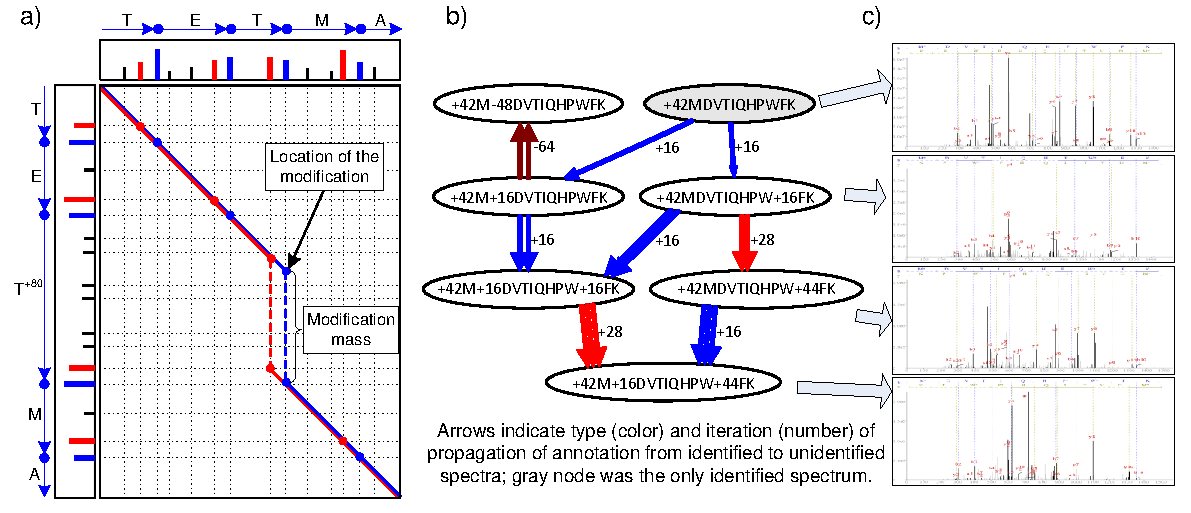
\includegraphics{figures/figSpectralNetworks.eps}}
\scalebox{0.8}{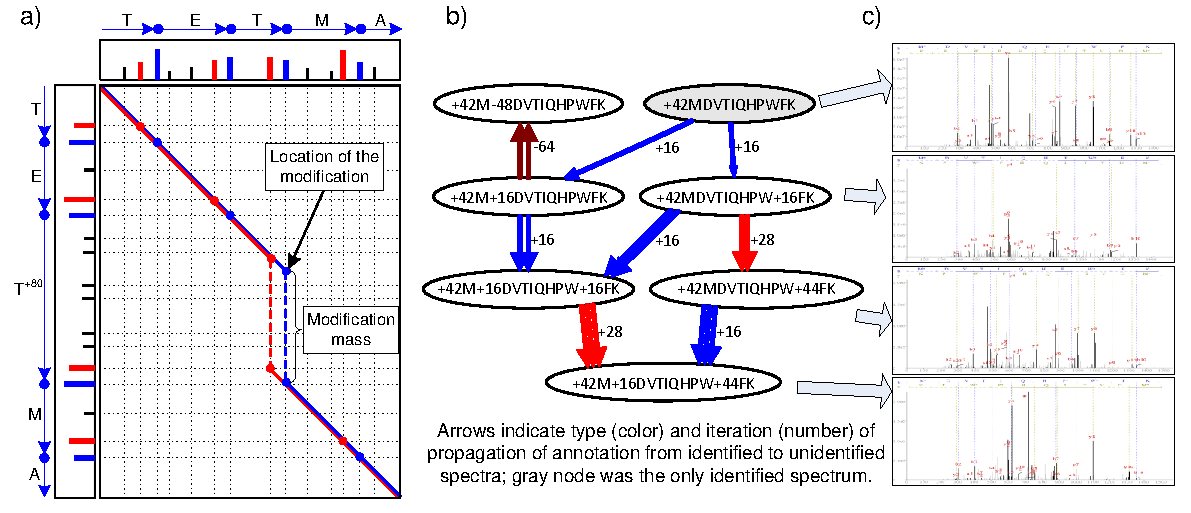
\includegraphics{figures/figSpectralNetworks.pdf}}

\caption{\footnotesize{\bf Identification of posttranslational modifications (PTMs) through spectral networks.} \textbf{a)} Spectral alignment between modified and unmodified variants of spectra from the peptide TETMA (prefix/suffix masses shown in blue/red, diagonal lines track consecutively matched masses); \textbf{b)} Grouped modification states of the peptide MDVTIQHPWFK from a sample of cataractous lenses; \textbf{c)} Highly correlated MS/MS spectra from the indicated peptide variants.}
\label{trd.snets.fig.spectralNetworks}
\end{figure}
\normalsize

%The second major limitation addressed in this TRD is that instead of identifying one spectrum at a time, our proposed spectral networks will detect and determine consensus identifications for {\em groups} of MS/MS spectra from related peptides (Figure~\ref{trd.snets.fig.sps}). High-throughput instruments typically generate spectra for multiple variants of each peptide~\cite{picotti07,nielsen06} and,
As we have shown in the previous CCMS cycle, %~\cite{bandeira07mcp,bandeira07pnas,bandeira08,bandeira08mann,gonzalez10,yang11,guthals12metasps},
correlations between multiple-aligned spectra can be used to dramatically increase signal-to-noise ratios and compensate for missing fragmentation by aggregating peaks from multiple spectra (Figure~\ref{trd.snets.fig.sps}). The resulting {\em consensus} interpretations for groups of spectra from related peptides (i.e., spectral networks) were shown to be a powerful tool in the discovery of  PTMs~\cite{bandeira07pnas,gonzalez10,yang11} with the ability to derive peptide sequences directly from  spectra (de novo sequencing) at unprecedent levels of accuracy~\cite{bandeira07mcp,guthals12metasps} and length~\cite{bandeira08,guthals12metasps}. Similarly to the assembly of DNA reads into genome sequences, these methods have enabled de novo spectral assembly of modified venom proteins~\cite{bandeira07mcp} %, database-assisted full-length monoclonal antibody sequencing~\cite{bandeira08},
%discovery of putative PTMs~\cite{bandeira07pnas,gonzalez10,yang11}
and integrated support for multi-stage mass spectrometry~\cite{bandeira08mann}.

\begin{figure}[htb!]
\centering
%  \includegraphics[height=15cm]{figures/figSPS.eps}
%  \scalebox{1.2}{\includegraphics{figures/figSPS.eps}}
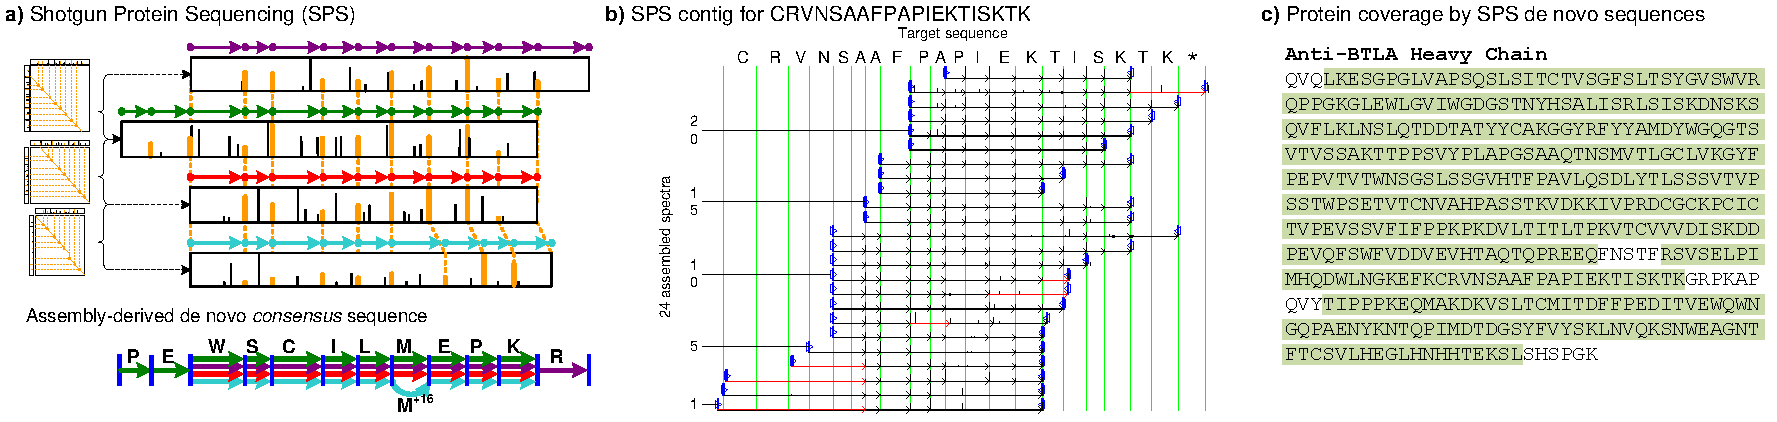
\includegraphics[width=\textwidth]{figures/figSPS.pdf}

  \caption{\footnotesize{\bf Shotgun Protein Sequencing (SPS) via assembly of tandem mass spectra.} \textbf{a)} Spectral alignment between spectra for peptide WSCILMEPKR (purple), PEWSCILMEPKR (green), WSCILMEPK (red), WSCILMoxEPK (cyan); Mox represents oxidized Methionine. Matching peaks in spectral alignments become pairwise gluing instructions between every pair of aligned spectra. \textbf{b)} Protein contig resulting from 24 spectra from a monoclonal antibody (aBTLA heavy chain). Each spectrum is shown superimposed with a sequence of arrows indicating its sequence of recovered masses; modified variants of the consensus sequence are indicated by red arrows (6 different modifications on 7 spectra). \textbf{c)} The nearly-complete aBTLA heavy chain sequence recovered by Comparative SPS~\cite{bandeira08}; highlighted sections were covered by protein contigs (95\% coverage) and the missing amino acids were obtained from homologous protein sequences.}
  \label{trd.snets.fig.sps}
\end{figure}

We further capitalized on homology between Shotgun Protein Sequencing (SPS) long/accurate {\em de novo} sequences and database sequences to deliver the first automated full-length protein sequencing approach (Comparative SPS~\cite{bandeira08}) and demonstrated it with database-assisted {\em de novo} sequencing of purified monoclonal antibodies. Spectral alignment algorithms also underlie the related CCMS work of Castellana~et~al.~\cite{castellana10,castellana11}, who proposed an effective method for sequencing monoclonal antibodies with database-guided iterative alignment+assembly of spectra from overlapping peptides. Both of these methods rely upon the existence of a homologous database. To reduce this dependence, we have since developed MetaSPS~\cite{guthals12metasps} algorithms for assembling SPS contigs into {\em meta-contigs} (sets of overlapping contigs). These methods now deliver {\em de novo} sequences over 100 AA long
that are 98\% accurate.

%at sequencing error rates as low as 1 mistake per 50 predicted amino acids without requiring homology to known sequences, which demonstrates the %feasibility of fully-automated {\em de novo} protein sequencing from mass spectrometry data. %It is expected that the performance of these algorithms %will only improve as new types of mass spectrometry data (e.g., Electron Transfer Dissociation) are also incorporated in SPS and spectral networks %approaches.

%*******************************************
\section{Innovation}
%*******************************************

% Why new developments are needed

%In the same way that BLAST and sequence alignment can be used for both database search and de novo shotgun sequencing, the proposed algorithms will also substantially extend current approaches for creating and searching spectral libraries. Spectral library search approaches have long been the standard approach in metabolomics mass spectrometry thanks to extensive efforts by the National Institute of Standards and Technology (NIST) in systematically accumulating reference spectra for very large collections of compounds. But even though peptide spectral library search also identifies significantly more spectra (e.g., 20-40\% more) than sequence database search when exploring the {\em exact same} search space, the core limitation to its widespread adoption has been that the libraries remain very small in comparison with the currently-known diversity of endogenous peptides. In a preliminary exploration of the space of currently-observable endogenous peptides, as determined by the number of observable distinct spectra, CCMS clustered 1.18 Billion spectra~\cite{frank11} acquired at Pacific Northwest National Lab over a period of 8 years from over 100 different species

We argue that overcoming the peptide identification bottleneck in proteomics
%, metaproteomics and peptidomics
will require new ways of thinking about  mass spectra in order to develop new ways of interpreting them. The spectral networks paradigm differs from the current mainstream paradigm in its  computation of consensus sequences for sets of spectra from related peptides, thus enabling applications where current paradigms perform poorly or completely fail.
%By finding spectra from related peptides even before considering their possible identifications and using these spectra to determine consensus identifications for {\em sets} of spectra from related peptides (instead of separately attempting to identify one spectrum at a time), the spectral networks paradigm addresses many pitfalls of mainstream tools.
In addition to improving peptide identification, molecular spectral networks further open up new computational avenues for analysis of
%natural products and
of non-peptidic molecules, including
% compounds with non-linear structures, unusual amino acids or rare post-translational modifications,
lipids, glycans, and other families of compounds. In the new cycle we propose to integrate and  scale spectral archives and spectral networks algorithms.

The 218 million clusters (of presumably unique peptides) resulting from CCMS's spectral archives analysis of 1 Terabyte of data already dwarf the currently available NIST peptide spectral libraries which only contain spectra for $\approx$850,000 peptides. It is expected that scaling this analysis $>$100-fold (to include all the data that will be available in the public domain during this project period)
 will further increase the number of observable unique peptides by at least 10-fold, for a total potential increase of up to $10\times\frac{218,000,000}{850,000}\simeq 2,500\times$ in the size of spectral libraries available for peptide identification . We propose to meet this challenge by developing new algorithmic and statistical approaches for construction (by identification) and searching of terabyte-scale spectral libraries, using both single-spectrum and spectral networks analysis.

Spectral networks differ from the mainstream database search paradigm for identification of MS/MS spectra by contesting its dogma that peptides should be identified by searching {\em one spectrum at a time} against a database of known protein sequences. We propose the following studies that deviate from this paradigm:
\begin{itemize}
%
\item Spectral networks find and group MS/MS spectra from related peptides and only then determine consensus interpretations for such {\em sets} of multiply-aligned spectra. Efficient hashing, limited de novo (sequence tags) and machine learning techniques will be used to construct networks for very large collections of spectra.
%
\item New algorithms will be developed to substantially improve peptide identification via spectral library search using rigorous p-value calculations and allowing for polymorphism-tolerant spectrum-spectrum matches.
%matching against spectral libraries (collections of previously-identified MS/MS spectra) while allowing for the co-occurrence of multiple peptides per spectrum (see Figure~\ref{figLibsSigs}d).
%
\item Our  new approach to spectrum-spectrum matching and peptide identification will be based on the concept of {\em spectral projections} - models of {\em differential} peptide fragmentation capturing correlated ion intensities in spectra of related peptides. Thus, we will {\em(i)} systematically characterize changes in MS/MS fragmentation patterns between spectra of related peptides and {\em(ii)} use these to define new spectrum-spectrum matching models.
%signatures from spectral network analysis of large datasets and {\em(ii)} use signatures for peptide identification by modeling each observed spectrum as a multiplexed composition of previously-known peptide and signature spectra.
%
\item We will develop a statistical framework based on rigorous calculation of theoretical p-values~\cite{kim08,gupta11}  to assess the significance of spectral networks search results.
% and integrated with existing tools to output identifications at predefined False Discovery Rates.
%
\item We will extend the CCMS-proposed concept of spectral dictionaries~\cite{kim09msdict} to spectral network dictionaries with the goal to construct and identify spectral networks.
%
\item We will develop new spectral alignment and spectral networks algorithms to create networks for spectra from any type of molecule.
\end{itemize}

%*******************************************
\section{Approach}
%*******************************************

%% Published results and spectral networks updates
%
%\begin{itemize}
%    \item Clustering and Spectral Archives: Spectral archives
%    \item Spectral libraries and matching/searching: M-SPLIT, NeuroPedia, MS-GF+ vs spectral library search comparison?
%    \item Spectral networks: Software engineering updates?, Pieter peptide specnets, Cancer, SILAC
%    \item Molecular networks: move to TRD on NRPs
%\end{itemize}
%
%{\em \bf Software engineering updates}
%\begin{figure*}[!htb]
%\centering
%%\scalebox{0.95}{\includegraphics{figures/figSpecNets.eps}}
%\caption{Software architecture of the C++ spectral networks code base}
%\label{trd.snets.fig.cpp}
%\end{figure*}


%\NeedRevision{\bf Spectral library matching.}
%%
%The repeated acquisition and reliable identification of MS/MS spectra %from a range of biological systems including various microbial species, mammalian tissues and cell lines
%has led to the accumulation of large collections of identified MS/MS spectra from mostly unmodified or modified peptide sequences. As a result, peptide identification by matching spectra of unidentified peptides against {\em spectral libraries} of identified peptide spectra~\cite{lam07} has recently gained new relevance, especially since the introduction of decoy spectral libraries~\cite{lam10} for calculation of false discovery rates~\cite{elias07,nesvizhskii10}. Searching against libraries of predicted spectra is also a promising emerging approach~\cite{yen09,yen11}.

%In addition to improving peptide identification, spectral library search opens up new possibilities for interpretation of MS/MS spectra. For example, mainstream approaches were developed under the ubiquitous assumption that each MS/MS spectrum is generated from a single peptide. While chromatographic procedures greatly contribute to making this a reasonable assumption, there are several situations where it is difficult or even impossible to separate pairs of peptides. Examples include certain permutations of the peptide sequence or PTMs (see~\cite{phanstiel08} for examples of co-eluting histone modification variants). In addition, innovative experimental setups have demonstrated the potential for increased throughput in peptide identification using mixture spectra - examples include Data-Independent Acquisition~\cite{venable04dia}, Ion-Mobility Mass Spectrometry~\cite{masselon03} and MS$^E$ strategies~\cite{chakraborty07}. To address the resulting computational bottleneck, we introduced the first spectral library-based approach (M-SPLIT~\cite{wang10}) for identification of mixture spectra generated from more than one peptide. Theoretical bounds were proposed to prune the search space using branch-and-bound techniques and further improved using a new projected-cosine metric. In brief, M-SPLIT uses single-peptide matches to prune the search space for mixture peptides - it first matches experimental spectra to single-peptide spectra and then attempts to improve the score of the match by adding more single-peptide matches to form mixture-spectrum matches (false discovery rates also controlled using decoy spectral libraries~\cite{lam10}). Thus, M-SPLIT dramatically reduces the search space by six orders of magnitude and is fast, even when searching against proteome-scale spectral libraries. Despite considering only a tiny fraction of the whole search space, benchmarks on both simulated and experimental data show that M-SPLIT~\cite{wang10} has both high sensitivity ($\approx$94\%) and high accuracy (up to $\approx$98\%).

%{\bf Clustering unidentified spectra.}
%%
%%The simplest example of a spectral network is the detection of MS/MS spectra from repeated acquisition of the same peptide in the same or multiple mass spectrometry runs; in these cases every node in the network is an individual spectrum in a separate run and edges between nodes indicate that the connected nodes represent spectra from the same peptide.
%Typically, in MS/MS analysis, each spectrum in the dataset is searched against a sequence database. At times, this can be very inefficient since MS/MS data sets contain many redundancies (it is common for peptides to get selected for fragmentation more than once~\cite{tabb03a}). When mass spectra are collected from several runs, such redundancies can add up to hundreds and even thousands of spectra from the same
%peptide. Instead of repeating the identification process for each spectrum, it can be beneficial to perform the search only once using a representative consensus spectrum per peptide and later apply the results to all similar spectra~\cite{tabb03a,beer04,tabb05}. By analyzing only representative spectra (one per cluster of spectra from each precursor mass), our MS-Cluster algorithm~\cite{frank08} scaled this approach for the analysis of tens of millions of spectra and resulted in a significant speed-up of MS/MS database searches (up to 10 fold) while simultaneously increasing the total number of identifications. Soon after, MS-Cluster was extended~\cite{frank11} to be able to process over $\approx$1.18 billion spectra acquired at Pacific Northwest National Lab over a period of 8 years. This extension served as the foundation for the proposed concept of {\em spectral archives}~\cite{frank11}, which extend spectral libraries by retaining both identified {\em and} unidentified spectra in the same way and maintaining information about peptide spectra that are common across species and conditions. Thus archives offer both traditional library spectrum similarity-based search capabilities along with new ways to analyze the data.

%\subsubsection*{Spectral networks for analysis of post-translational modifications}
%
%Samples of digested proteins often contain multiple overlapping peptides covering the same region of a protein sequence, such as prefix peptides (e.g. PEPTI/PEPTIDES), suffix peptides (e.g. TIDES/PEPTIDES) or partially-overlapping peptides (e.g. PEPTIDES/TIDESHIGH). In addition, most experimental protocols unintentionally generate multiple chemical modifications (e.g., oxidation) and it has been repeatedly shown that existing MS/MS datasets typically contain modified versions for many peptides~\cite{Hunyadi-Gulyas04, tanner05,tsur05,Wilmarth06}.
%%
%If the peptide sequences were known in advance, determining their overlap would be a straightforward application of the standard sequence alignment algorithms~\cite{smith81}. Conversely, spectral alignment is defined as the alignment of matching peaks between spectra from overlapping peptides~\cite{pevzner00,bandeira06}. This concept is illustrated in \mbox{Figure~\ref{figSpecNets}a} with the matching $b$-ions highlighted in blue. The surprising outcome of spectral alignment, as opposed to sequence alignment, is that even though one does not know the peptide sequences in advance, the sequence information encoded in the masses of the $b$/$y$-ions actually suffices to detect pairs of MS/MS spectra from overlapping peptides. In fact, it turns out that the reliability of spectral alignment allows one to discern the high-scoring true spectral pairs from the many millions of possible spectral pairs in high-throughput proteomics experiments~\cite{bandeira06,bandeira07pnas}. Moreover, since each spectrum may align to several other spectra, the set of detected spectral pairs defines a \emph{spectral network} where each node corresponds to a different spectrum and nodes are connected by an edge if the corresponding spectra were found to to be significantly aligned. This concept is illustrated in \mbox{Figure~\ref{figSpecNets}b-c} with spectral networks from human cataractous lens~\cite{bandeira07pnas} and a monoclonal antibody raised against the B- and T-cell lymphocyte attenuator molecule~\cite{bandeira08}. Note that since most spectra usually come from non-contiguous protein regions, the consequent outcome of this approach is not a single spectral network but rather multiple spectral networks, one for each set of spectra from overlapping peptides.
%
%In traditional DNA sequence alignment, it often happens that query sequences differ from the reference sequences by the insertion or deletion of one or more nucleotides~\cite{smith81}. While the insertion/deletion of amino acids is also usually allowed when aligning protein sequences, an additional factor needs to be considered when aligning peptides from experimental samples due to the occurrence of post-translational modifications. %In fact, multiple groups have shown~\cite{tsur05,savitski06,na11} that the phenomenon of unexpected modifications is much more widespread than commonly acknowledged.
%%
%From a sequence alignment perspective, a modification could be modeled by following the modified residue with a special character for each type of modification. Thus, the alignment of a modified peptide PEPT*IDE with its unmodified counterpart PEPTIDE would result in a single difference caused by the insertion of the modification `*'.
%%
%In tandem mass spectrometry, however, a modification of mass $m$ conceptually corresponds to the insertion of additional $m$~Da in the $b$/$y$-ion series between the ions immediately preceding and following the site of post-translational modification ({\em i.e.} the mass of the residue becomes larger by mass $m$). Conversely, if the modification causes a loss of $m$~Da from the modified residue then the corresponding effect is the subtraction of $m$~Da between the ions for the modified residue. When applied to unmodified and modified versions of the same peptide, the role of spectral alignment algorithms~\cite{pevzner01,bandeira04,bandeira07pnas} is to $a$) use the spectrum of the unmodified peptide to determine where to position the modification mass in the spectrum of the modified peptide and $b$) to assess whether the post-alignment match between the two spectra is significant enough to accept the spectra as a pair of modified/unmodified spectra from the same peptide. Thus, spectral alignment considers every possible spectral pair and every possible location for the mass difference ({\em i.e.} modification mass) between the aligned spectra. Figure~\ref{figSpecNets}a illustrates the spectral alignment between MS/MS spectra from the peptides TETMA and phosphorylated TET$^{+80}$MA. By requiring a significant match between the aligned spectrum peaks~\cite{bandeira07pnas} and by placing no restrictions on which modifications to consider, this approach can be used to discover novel or unexpected modifications. In fact, when applied to a set of spectra from cataractous lenses proteins from a 93-year old patient, spectral networks were able to rediscover the modifications identified by database search methods and additionally discovered several novel modification events~\cite{bandeira07pnas,tsur05}.
%
%\begin{figure*}[!htb]
%\centering
%\scalebox{0.95}{\includegraphics{figures/figSpecNets.eps}}
%\caption{Discovery and identification of post-translational modifications through spectral networks; \textbf{a)} Spectral alignment between modified and unmodified variants of the peptide TETMA ($b$-ions shown in blue, $y$-ions in red, blue/red lines track consecutively matched $b$/$y$-ions); \textbf{b)} Grouped modification states of the peptide MDVTIQHPWFK from a sample of cataractous lenses. Nodes in the spectral network represent individual MS/MS spectra and edges between nodes represent significant spectral alignments such as that shown in part (a); \textbf{c)} Spectra assembled in the spectral network for TNSMVTLGCLVK with diverse Cysteine modifications on a monoclonal antibody. Each arrow corresponds to the propagation of a sequence and/or PTM from an identified spectrum to an unidentified spectrum (repeated arrows are iterative propagations). Arrow colors correspond to types of modifications transferred.}
%\label{figSpecNets}
%\end{figure*}
%
%When first analyzing a sample possibly containing modified peptides one does not know a priori which residues or peptides will be modified. Thus, spectral alignment considers every possible spectral pair and every possible location for the mass difference (e.g. modification mass) between the aligned spectra. By requiring a significant match between the aligned spectrum peaks~\cite{bandeira07pnas} but placing no restrictions on which modifications to consider, this approach can be used to discover novel or unexpected modifications. In fact, when applied to a set of spectra from cataractous lenses proteins from a 93-year old patient, spectral networks were able to rediscover the modifications identified by database search methods and additionally discovered several novel modification events~\cite{tsur05,bandeira07pnas} (~\ref{figSpecNets}).
%
%The identification of peptides containing multiple modifications via database search is a challenging problem imparted by the combinatorial explosion in the number of possible modification variants for all the peptides in a database~\cite{tsur05,na11}. Not only can this make the approach much slower, but the increased number of peptide candidates for any given spectrum significantly increases the risk of incorrect identifications. However, samples containing peptides with two or more modifications often also contain variants of the same peptide with only one or no modification. In these cases, we have found that spectral alignment is able to group these related spectra from multiple modification variants of the same peptide into small spectral networks thus increasing confidence in their identity as a related peptide. Figure~\ref{figSpecNets}b illustrates the spectral network for a particular peptide in a sample of cataractous lenses proteins.
%
%By grouping together spectra from multiple variants of the same peptide, spectral networks additionally contribute to the reliable identification of highly modified peptides. While database searching is restricted to matching ion masses between theoretical and observed spectra, spectral networks further capitalizes on the occurrence of common fragment ions at corresponding masses with similar peak intensities (Figure~\ref{figSpecNets}c). In general, it becomes easier to identify a highly modified peptide if one additionally observes highly-similar spectra from its intermediate modification states. Thus, spectral alignment not only allows one to \emph{discover} unexpected modifications (instead of only identifying expected modifications) but additionally provides an alternative route for identification of highly modified peptides.

%\subsubsection*{Shotgun Protein Sequencing}

%Current approaches to proteomics focus on the reliable identification of proteins under the assumption that all proteins of interest are known and present in a database. However, the limited availability of sequenced genomes and multiple mechanisms of protein variation often refute this assumption. Well known mechanisms of protein diversity include variable recombination and somatic hypermutation of immunoglobulin genes~\cite{gearhart02}. The vital importance of some of these novel proteins is directly reflected in the success of monoclonal antibody drugs such as Rituxan\texttrademark, Herceptin\texttrademark and Avastin\texttrademark~\cite{wiles06,haurum06,bandeira08}, of which all are derived from proteins that are not directly inscribed in any genome. Similarly, multiple commercial drugs have been developed from proteins obtained from species whose genomes are not known. In particular, peptides and proteins isolated from venom have provided essential clues for drug design~\cite{lewis03,pimenta05} - examples include drugs for controlling blood coagulation~\cite{joseph04,swenson04a,kini01} and therapeutic treatments for breast~\cite{swenson04,pal02} and ovarian~\cite{markland01} cancer. Despite this vital importance of novel proteins, the mainstream method for protein sequencing is still initiated by restrictive and low-throughput Edman degradation~\cite{ZugastiCruz06,ogawa04} - a task made difficult by protein purification procedures, post-translational modifications and blocked protein N-termini. These problems gain additional relevance when one considers the unusually high level of variability and post-translational modifications in venom proteins~\cite{buczek05,pimenta05a}.
%
%Conceptually, sequencing a protein from a set of MS/MS spectra can be described by a simple analogy. Imagine a jewelry box with many identical copies of a specific model of bead necklaces. Although all the beads are identical, this model is characterized by having irregular distances between consecutive beads \-- the set of inter-bead distances is initially chosen by the designer and all necklaces are then made using exactly the same specification. Now assume that one day you open your jewelry  box and realize that someone has vandalized all the necklaces by cutting them to fragments at randomly chosen bead positions. Can you recover the original design of this model of necklaces, as specified by the set of consecutive inter-bead distances? In this allegory inter-bead distances correspond to amino acid masses and beads correspond to MS/MS fragmentation points (between consecutive amino acids). MS/MS data add more than a few difficulties to this necklace assembly problem; for example, most peaks in MS/MS spectra do not correspond to any fragment ions (extra beads) and many fragment ions do not result in any peaks (missing beads). Nevertheless, Figure~\ref{figSPS} presents an example of assembled MS/MS spectra resulting in a 22 amino acid long segment of a monoclonal antibody~\cite{bandeira08}.
%
%\begin{figure}[htb!]
%\centering
%%  \includegraphics[height=15cm]{figures/figSPS.eps}
%  \scalebox{1.2}{\includegraphics{figures/figSPS.eps}}
%  \caption{Shotgun Protein Sequencing (SPS) via assembly of tandem mass spectra; \textbf{a)} Spectral alignment between spectra for peptide WSCILMEPKR (purple), PEWSCILMEPKR (green), WSCILMEPK (red), WSCILMoxEPK (cyan); Mox represents oxidized Methionine. Matching peaks in spectral alignments become pairwise gluing instructions between every pair of aligned spectra. \textbf{b)} Protein contig resulting from 24 spectra from a monoclonal antibody (aBTLA heavy chain). Each spectrum is shown superimposed with a sequence of arrows indicating its sequence of recovered masses; modified variants of the consensus sequence are indicated by red arrows (6 different modifications on 7 spectra). \textbf{c)} The complete aBTLA heavy chain sequence recovered by Comparative SPS~\cite{bandeira08}; highlighted sections were covered by protein contigs (95\% coverage) and the missing amino acids were obtained from homologous protein sequences.}
%  \label{figSPS}
%\end{figure}
%
%Shotgun Protein Sequencing ({\em SPS}) is a {\em de novo} sequencing approach~\cite{bandeira04} that utilizes multiple MS/MS spectra from overlapping peptides generated using non-specific proteases or multiple proteases with different specificities~\cite{johnson87,klammer06,englander03,maccoss02a,pham06}. The original approach was based on the overlap~$\rightarrow$~layout~$\rightarrow$~consensus approach to assembly and shown to be efficient for the assembly of a single purified unmodified protein. However, practical applications (like sequencing snake venoms) require applicability to mixtures of modified proteins. In fact, most MS/MS samples contain both modified and unmodified versions for many peptides, including biological and chemical modifications both native and introduced during sample preparation. Sequence variations and post-translational modifications present a formidable algorithmic challenge for assembly algorithms as the performance of the original SPS approach~\cite{bandeira04} steeply degraded as soon as even a small percentage of the spectra are from modified peptides. To use the beads analogy, the necklace puzzle becomes very difficult if in addition to the canonical necklaces (non-modified proteins), the jewelry box also contains some necklaces that deviate from the designer's specification (modified proteins). Building on spectral networks algorithms for analysis of post-translational modifications based on alignment of spectra from modified and unmodified peptide variants~\cite{bandeira06,bandeira07pnas}, we showed how to integrate these alignments into Shotgun Protein Sequencing to derive a completely new form of spectral assembly. This utilized a generalized notion of {\em ABruijn~graphs} (originally proposed in the context of DNA fragment assembly~\cite{pevzner04}) for the assembly of MS/MS spectra from overlapping, modified and unmodified peptides into {\em contigs} (sets of aligned spectra from overlapping peptides, see Figure~\ref{figSPS}), where each contig then capitalizes on the corroborating evidence from the assembled spectra to yield a high-quality {\em consensus} {\em de novo} sequence. As a result, SPS consensus {\em de novo} sequences were found to be twice as accurate as sequences derived from single spectra (1 mistake per 10 vs 5 amino acid predictions) while yielding sequences that were much longer that single-peptide/spectrum could support (up to 24 AA long).
%
%Recently this paradigm was extended in two distinct directions. First, we capitalized on homology between SPS long/accurate {\em de novo} sequences and known sequences to deliver the first automated full-length protein sequencing approach (Comparative SPS~\cite{bandeira08}) and demonstrated it with database-assisted {\em de novo} sequencing of two monoclonal antibodies. Spectral networks also underlie the related work of Castellana et al.~\cite{castellana10,castellana11}, who proposed an effective method for sequencing monoclonal antibodies with database-guided iterative alignment+assembly of spectra from overlapping peptides. Both of these methods rely upon the existence of a homologous database. To reduce this dependence, we have since developed MetaSPS~\cite{guthals12metasps} algorithms for assembling SPS contigs into {\em meta-contigs} (sets of overlapping contigs). These methods now deliver {\em de novo} sequences over 100 AA long at sequencing error rates as low as 1 mistake per 50 predicted amino acids without requiring homology to known sequences, which demonstrates the feasibility of fully-automated {\em de novo} protein sequencing with unidentified MS/MS spectra. It is expected that the performance of these algorithms will only improve as new types of mass spectrometry data (e.g., Electron Transfer Dissociation) are also incorporated in SPS and spectral networks approaches.

\subsection{Aim 1: Prediction and matching of tandem mass spectra using spectral projections}

Generative statistical models of MS/MS peptide fragmentation have long been used to implicitly ``predict'' theoretical MS/MS spectra used to score peptide spectrum matches in de novo sequencing~\cite{dancik99} and database search~\cite{kim09msdict,kim10cidetd}. Despite substantial ongoing efforts~\cite{wysocki03,zhang04,paizs05}, the core rate-limiting step of predicting theoretical MS/MS spectra from peptide sequences remains a challenging open problem. While some of the most sophisticated tools for scoring Peptide-Spectrum Matches seem to avoid this issue~\cite{kall07,kim08}, including many CCMS tools~\cite{kim08,kim09msdict,frank09ranks,kim10cidetd,wang11}, a closer look reveals that their statistical models of ion fragmentation still essentially encode for or are explicitly based on predictive models of what a theoretical spectrum should look like. In difference from these, we propose a new {\em spectral projection} approach for prediction of peptide spectra and scoring of spectrum-spectrum matches. Instead of predicting a tandem mass spectrum from a peptide sequence (a key limitation in current approaches), spectral projections use one or more spectra from related peptides to generate the spectrum for the peptide of interest.

Similarly to the power of genomics sequence homology to detect related sequences within and across species, we have found that spectra of peptides with related sequences also share substantial ``spectrum homology'' \--- that is, the relative abundances of the spectrum peaks tend to be highly correlated after correcting for the expected shifts in fragment masses. As shown in Fig.~\ref{trd.snets.fig.projections}a for different amino acid substitutions ({\em polymorphism variations}) and in Fig.~\ref{trd.snets.fig.spectralNetworks}c for multiple PTMs ({\em PTM variations}), these correlations can be as high as are typically observed between multiple spectra from the same peptide - a key observation since these variations are one of the major reasons for low spectrum identification rates in both singles-species~\cite{nielsen06,picotti07}, multi-species (e.g., microbiome or other metaproteomics samples, see Figure~\ref{trd.snets.fig.shewanella}) or polymorphic~\cite{shevchenko03,habermann04} (e.g., cancer) proteomics analysis.
%
Spectral projections will test the hypothesis that prediction of MS/MS spectra can be significantly improved by taking MS/MS spectra of identified peptides and {\em projecting} them into spectra of previously-unobserved peptides. Preliminary results demonstrate the feasibility of this approach (Fig.~\ref{trd.snets.fig.projections}) and multiple strategies will be applied to further maximize the chances of success.
%
Spectral projection models will be derived from the systematic characterization of correlated peptide fragmentation and will be used to address three core problems: {\em (i)} to predict peptide spectra from other spectra instead of sequences, {\em (ii)} to extend spectral library search for identification of similar but previously-unobserved peptides and {\em (iii)} to `blindly' detect pairs of unidentified spectra differing by a known type of variation.

\begin{figure}[!t]
\small
\centering
%\scalebox{0.7}{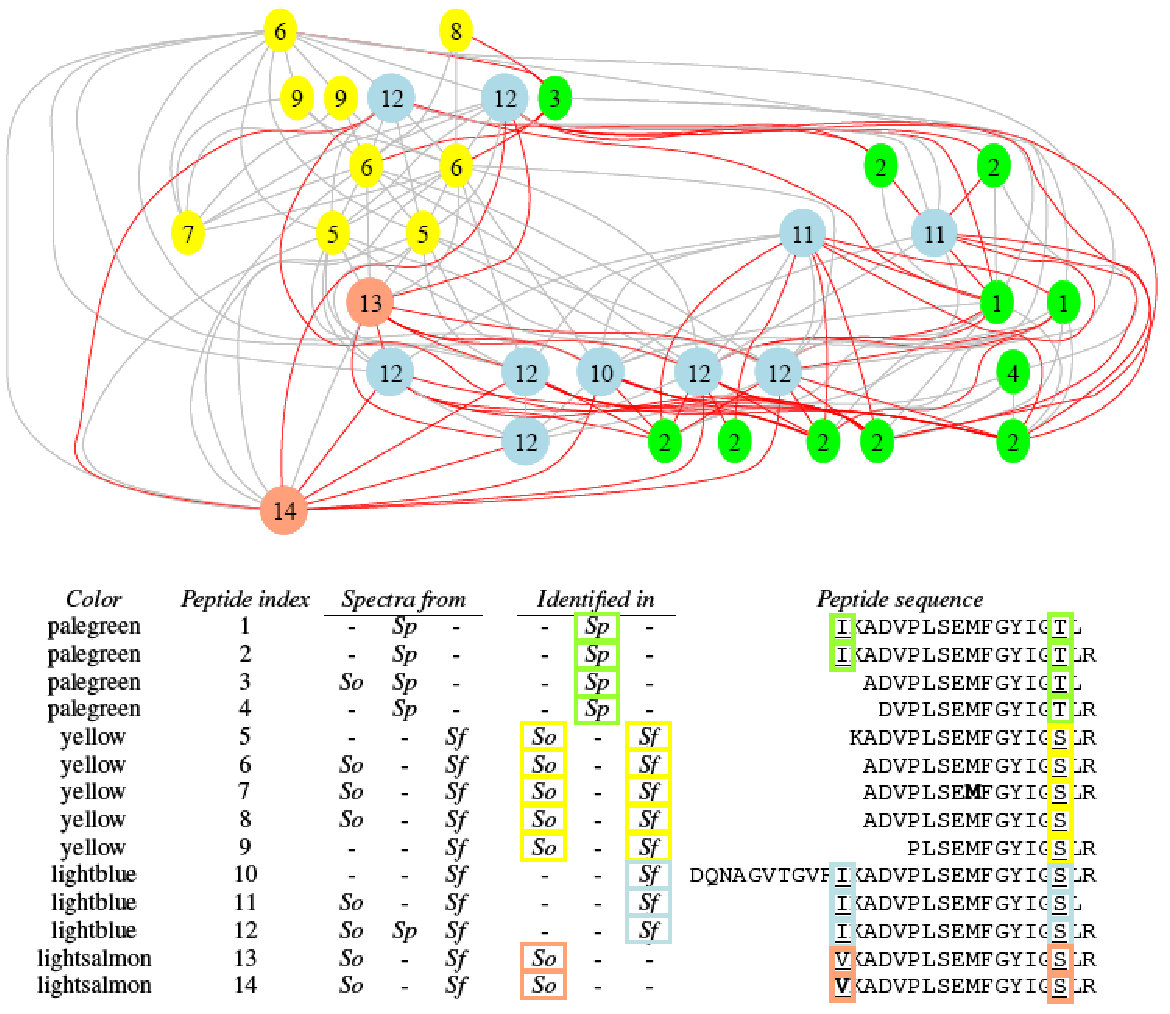
\includegraphics{figures/figShewanella.eps}}
\scalebox{0.8}{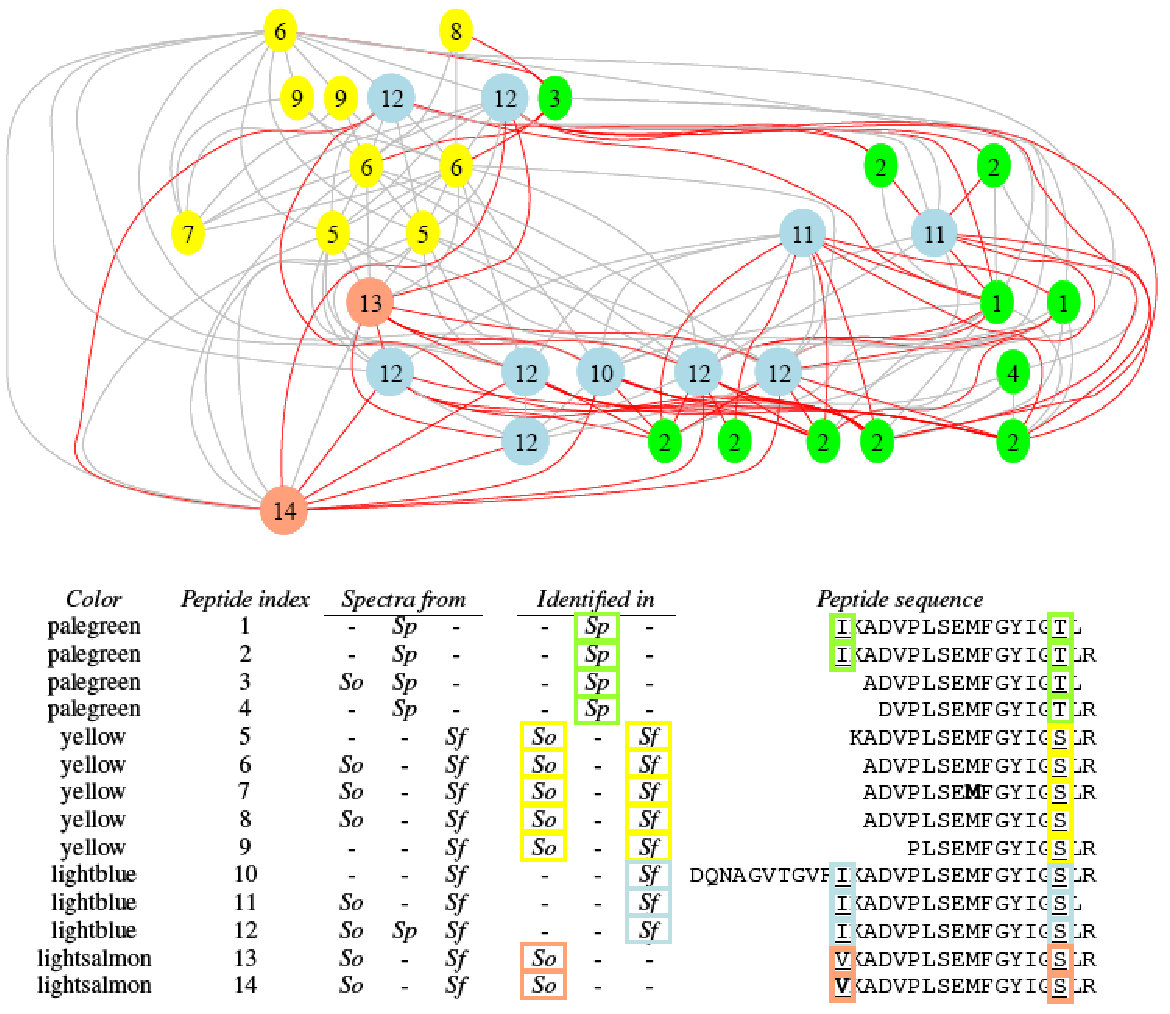
\includegraphics{figures/figShewanella.pdf}}

\caption{\footnotesize{\bf Multi-species spectral network with species-specific mutations}. Vertices in the spectral network represent aligned spectra: colors indicate species contexts where each spectrum was found and numbers indicate different sequences, as shown in the table. Edge colors represent type of spectral pair: gray = prefix/suffix or PTM variations, red = mutation/polymorphism variations. \emph{``Spectra from''} indicates which species contained each spectrum; \emph{``Identified in''} indicates which databases contain the identified sequence. The network reveals two mutated sites I/V towards the beginning of half the peptides and T/S towards the end of all peptides. %According to the current {\em Shewanella} genomes,
All three observed combinations correspond to different species: I/T peptides are specific to {\em Shewanella putrefaciens (Sp)}, I/S peptides are specific to {\em Shewanella frigidimarina (Sf)} and V/S peptides are specific to {\em Shewanella oneidensis (So)}. However, the fact that peptides 11-14 were identified from spectra obtained from both {\em So} and {\em Sf} suggests that this variation also occurs intra-species (note that both I/V and T/S mutations could be caused by a single nucleotide polymorphism).}
\label{trd.snets.fig.shewanella}
\end{figure}
\normalsize

%This proposal aims to overcome the limitations of mainstream computational approaches to the identification of MS/MS spectra by challenging two fundamental dogmas that have dominated the field for over 40 years. The first dogma is that MS/MS spectra should be identified by matching against peptide sequences extracted from a protein sequence database derived from the corresponding genome.

%{\bf We propose a new {\em spectral projection} approach for prediction of peptide spectra}: instead of predicting a spectrum from a peptide sequence, {\bf spectral projections use a spectrum from a related peptide to generate the spectrum of the peptide of interest}.

A spectral projection from a spectrum $S$ into a spectrum $S_p$ is an operation that i) selects a subset of peaks from $S$, $ii$) modifies the m/z and intensity values of the selected peaks and $iii$) defines $S_p$ as the modified set of selected peaks. To assess the potential of this approach, we acquired MS/MS spectra for synthetic peptides containing many pairs of peptides whose sequences differed by one amino acid substitution (in collaboration with Antonius Koller at SUNY Stony Brook). Using these two datasets, one for peptides of length 5 and another for peptides of length 14, we investigated the correlation of peak intensities for pairs of MS/MS spectra from $\approx 4,500$ unique peptides differing by just one amino acid. As shown in Fig.~\ref{trd.snets.fig.projections}, we found a striking pattern of highly correlated peak intensities: certain amino acid substitutions essentially result in a mass shift at the site of the substitution but seem to have a negligible effect on the relative intensities of MS/MS peaks. In fact, this intensity-preserving property sometimes holds even when there are two amino acid substitutions (Fig.~\ref{trd.snets.fig.projections}a).
%As expected, there are also cases where the amino acid substitution does significantly influence the relative peak intensities, such as most of the substitutions involving PHRK, which are known to imprint marked peptide fragmentation signatures in CID MS/MS spectra~\cite{gucinski10}.
%
As such, while a naive mass-shift spectral projection (i.e., change peak mass values according to the amino acid substitution but do not change peak intensities) would work between certain pairs of amino acids, it would fail on cases where the substitution does significantly influence the relative peak intensities, such as most of the substitutions involving Pro, His, Arg or Lys (all known to impact peptide fragmentation signatures in CID MS/MS spectra~\cite{gucinski10}).
%
%on the bottom-right in Fig.~\ref{trd.snets.fig.projections}. The results were very similar for the set of peptides of length 12 (data not shown), with 10 amino acid substitutions having only a small effect on relative peak intensities and revealing A/P as the single outlier substitution with highly pronounced changes to the intensity of peaks adjacent to the substitution site. This was not surprising since Proline (P) is known to imprint a marked peptide fragmentation signature in CID MS/MS spectra~\cite{breci03}.
%The examples illustrated in Fig.~\ref{trd.snets.fig.projections} suggest that even a simple mass-shift spectral projection whose only effect is to change the peak mass values according the amino acid substitution (no changes to peak intensities) would work for substitutions between certain pairs of amino acids. However, this particular spectral projection is limited in scope and expected to fail in a variety of relevant cases such as K/R (illustrated in Fig.~\ref{trd.snets.fig.projections}, light-blue arrow with a black label) and X/P, where X indicates any other amino acid.
%
We will use linear models of spectral projections to predict spectra for a range of possible {\em variations}: amino acid substitutions, posttranslational modifications and short sequence extensions/reductions.
%
As described below and illustrated in Fig.~\ref{trd.snets.fig.projections}d for A/P substitutions, linear models can yield projected spectra as similar to the corresponding experimental spectra as replicate spectra of the same peptides are similar among themselves.
%
%, different numbers of peptide charges and MS2/MS3 levels of peptide fragmentation}.
Spectra differing by one or more such variations will be analyzed in multiple mass spectrometry modes and specific spectral projections will be derived for CID, ETD and HCD fragmentation technologies. %each type of peptide fragmentation: CID (Collision-Induced Dissociation), ETD (Electron-Transfer Dissociation) and HCD (Higher-energy Collision Dissociation).

%Thus, there is a pressing need to determine projection models for specific spectrum changes resulting from different types of variations, which can be used for a) prediction and b) scoring. In some cases multiple types of variations may be captured by the same type of projection (e.g., those captured by the naive mass-shift projections) but others may be variation-specific (such as X/P). Also, some changes may be local (e.g., A/P results) while others are global (phos, immonium ions, different precursor charge-states).

%\begin{figure}[!tb]
%\small
%\centering
%\scalebox{0.7}{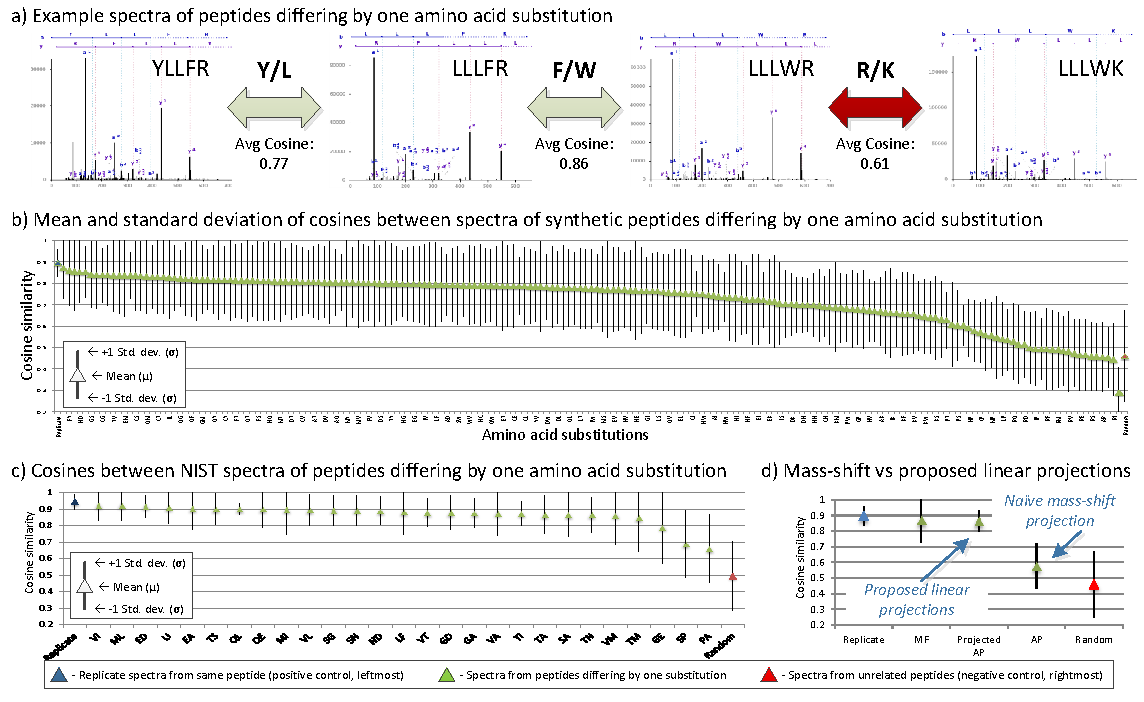
\includegraphics{figures/figProjections.eps}}
%\caption{\small{\bf MS/MS spectra of peptides differing by one or two amino acids.} Peptide sequences are indicated in boxes overlapped with the spectrum images; light/dark-blue arrows indicate spectra from peptides whose sequences differ by one/two amino acid substitutions, respectively; arrow labels in red/black indicate amino acid substitutions with little/pronounced effect on relative peak intensities, respectively. The dominating presence of red labels, even when associated with double amino acid substitutions, strongly suggests that spectra of unknown peptides can be predicted from spectra of known peptides using spectral projections. In fact, only two of the six peptide spectra shown here would suffice to obtain representative spectra for the other four - using a simple spectral projection to just shift the masses of peaks according to the amino acid substitution, one can start from either LLLWR or LLLWK and predict very high quality spectra for other four peptides (cosine similarity $\geq$0.9).}
%\label{trd.snets.fig.projections}
%\end{figure}

\begin{figure}[!tb]
\small
\centering
%\scalebox{0.85}{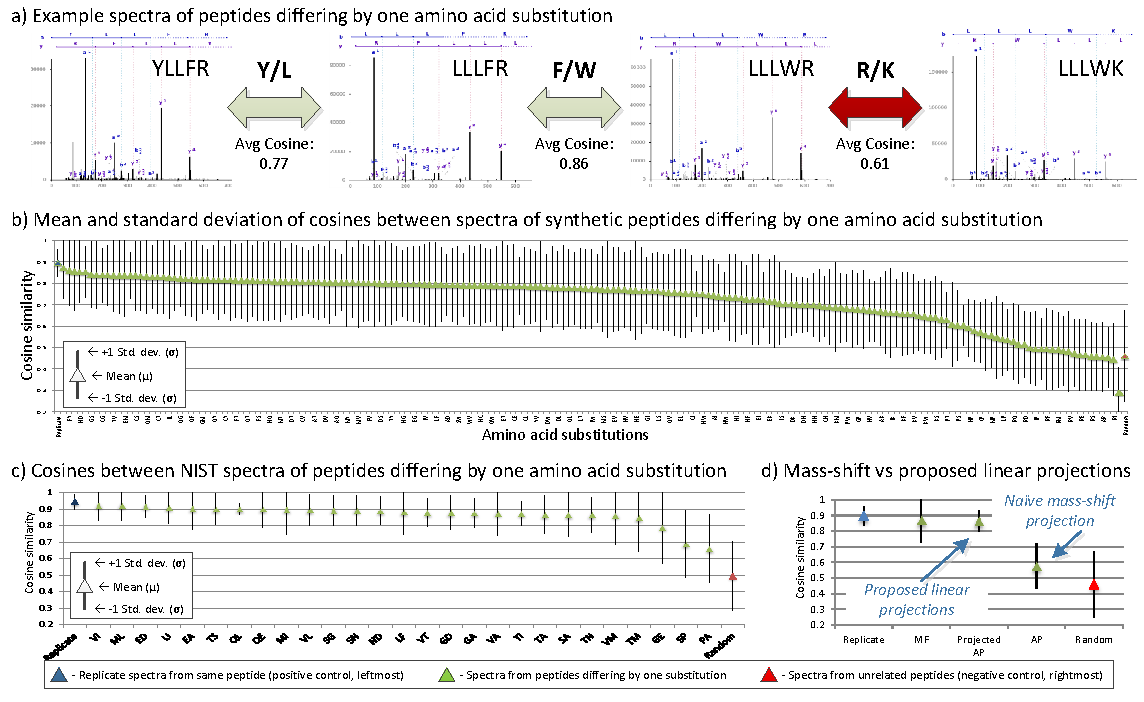
\includegraphics{figures/figProjections.eps}}
\scalebox{0.87}{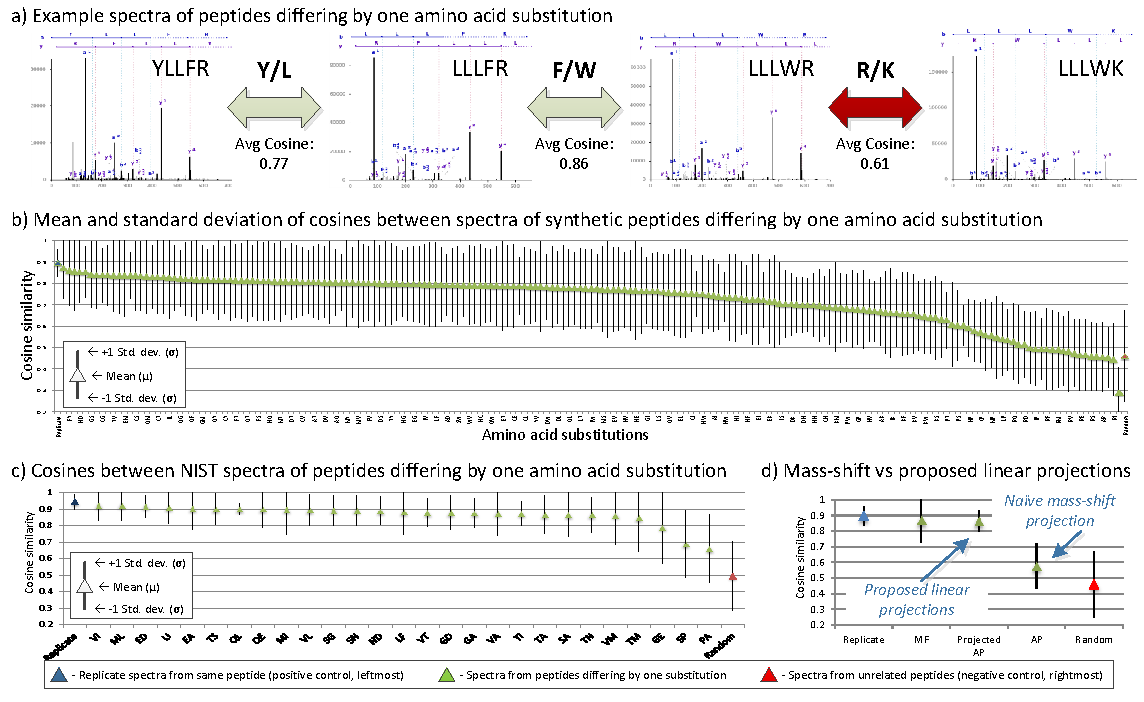
\includegraphics{figures/figProjections.pdf}}
\caption{\footnotesize{\bf Preliminary data supporting feasibility of spectral projections.} Cosines between MS/MS spectra were calculated by shifting peak masses according to each substitution without changing peak intensities.
%The markers and interval lines on parts b-d indicate mean and standard deviations of cosines ($y$-axis) between amino acid substitutions; the leftmost (blue) and rightmost (red) markers indicate the cosines between replicate spectra of the same peptide (positive control) and randomly matched peptides of the same length (negative control), respectively.
{\bf a)} Spectra of four peptides differing by single amino acid substitutions; green/red arrows indicate high/low similarity. {\bf b)} Systematic characterization of all possible single amino acid substitutions using a combinatorial library of synthetic peptides of length 14 with the substitution on position 7 and up to 128 unique spectrum pairs per substitution (using the synthesis pattern [DW][EL][FH]ST[VQ]X[AN]TSY[GW][EY]K, where $[]$ indicates a choice of amino acids and $X$ represents any amino acid). While many substitutions result in significantly similar spectra, many are not significantly different from the negative controls.  {\bf c)} Although only $\approx15\%$ of all $\frac{20\times 19}{2}=190$ substitutions can be assessed using NIST libraries (10+ spectrum pairs per subst.), the trends are similar between synthetic and NIST spectra for the same substitutions. {\bf d)} Modeling substitutions of $A\rightarrow P$ using the proposed linear projection models results in significantly higher similarity spectra than the naive mass-shift projection.}
\label{trd.snets.fig.projections}
\end{figure}

\normalsize

%-------------------------------------------------------------------------------------
\subsubsection{Generating datasets to train spectral projection models}\label{trd.snets.aim.sp.models}
%-------------------------------------------------------------------------------------

Determination and validation of spectral projection models will require large datasets of reliably-identified {\em pairs} of peptide spectra. Ideally the spectral projection model for each type of variation should be determined using many pairs of spectra from peptides differing only by that type of variation. %(e.g., PEPTIDE/PEPT$^{+80}$IDE, PRTEIN/PRT$^{+80}$EIN, etc).
%The exact definition of "many pairs of spectra" will depend on the complexity of the projection model - since the goal is to avoid over-fitting the model to a specific training set of spectral pairs, higher complexity models with more parameters will likely require more spectral pairs than simpler models. For example, the simple mass-shift projection described above requires no training because the peak intensities do not change and the mass shifts are directly determined from the mass of the variation.
%
Thus, we will collect identified peptide spectra from our collaborators, public repositories~\cite{falkner06,desiere06,craig06,martens05} and NIST spectral libraries~\cite{speclibNist}, altogether totaling over 2 Billion spectra from over 100 species including bacteria, yeast, arthropoda, plants, reptiles and mammals.

If these spectra do not suffice to determine certain projection models and to define `ground truth' validation datasets, we will also use low-cost combinatorial peptide synthesis to generate many pairs of spectra {\em for any variation of interest}. This approach was also applied in the analysis of phosphorylation sites~\cite{aguiar10} and we recently used it to improve identification of SUMOylated~\cite{wang12sumo} and cross-linked~\cite{wang12xlink} peptides by up to 400\% and 250\%, respectively.
%Combinatorial synthesis consists of allowing multiple amino acid choices at each step of peptide synthesis.
For example, a combinatorial peptide sequence "[AC][DEF]G[HK]" means that the first amino acid could be either A or C, the second could be D, E of F and the last could be either H or K, for a total of $2\times 3\times 1\times 2=12$ possible peptides from a single synthesis experiment. To assess the utility of this approach, we generated the preliminary data in Fig.~\ref{trd.snets.fig.projections}a from a prototype combinatorial peptide library generated with the sequence pattern [YWITV][GASKL][GASKL][FWITH][MRSKE] (maximum peptide diversity is $5^5=3,125$ distinct peptides). Since short peptides are difficult to identify in typical proteomics experiments, this library is a clear example of how synthesis can be used to overcome limitations of available datasets. To further maximize the utility and minimize the cost of combinatorial peptide synthesis, we will develop algorithms to maximize the number of new variations obtainable per sequence pattern.

%-------------------------------------------------------------------------------------
\subsubsection{Spectral projection models for prediction of MS/MS spectra of novel peptides}\label{trd.snets.aim.sp.proj}
%-------------------------------------------------------------------------------------

The analysis of many pairs of spectra differing by each type of variation will be used to determine linear models of spectral projection which will be integrated into a new spectrum prediction tool capable of predicting spectra for novel peptides.
%Maximizing similarity between predicted and real spectra will require the development of multiple spectral projection models for different types of variations, all of which {\bf will extend the naive mass-shift projection model to also predict changes in peak intensities}.
%
Linear projections can be described with a simple example of projecting a spectrum $S$ from PEPTIDE to a spectrum $S_p$ for PEPTADE. Let $v(S)$ represent the peak intensities for all N/C-term ions in $S$; considering only $b$/$y$-ions would yield $v(S)=(b_1,\ldots,b_6,y_1,\ldots,y_6)$, where each position in the tuple contains the peak intensity at the corresponding ion mass in $S$. A linear projection model for converting $I$ to $A$ at position 5 on a peptide of length 7 would correspond to $M^{I\rightarrow A}_{5,7} v(S) + A^{I\rightarrow A}_{5,7}$, where $M^{I\rightarrow A}_{5,7}$ is a multiplicative vector term of expected fold changes in ion intensities and $A^{I\rightarrow A}_{5,7}$ is an additive vector term of expected offsets in ion intensities. The projected spectrum $S_p$ is then defined using $v(S_p) = M^{I\rightarrow A}_{5,7} v(S) + A^{I\rightarrow A}_{5,7}$ by placing the $v(S_p)$ peak intensities at the theoretical $b$/$y$ ion masses for PEPTADE. Using

\begin{eqnarray*}
M^{I\rightarrow A}_{5,7} & = & (m^b_1,\ldots,m^b_6,m^y_1,\ldots,m^y_6) \\
A^{I\rightarrow A}_{5,7} & = & (a^b_1,\ldots,a^b_6,a^y_1,\ldots,a^y_6)
\end{eqnarray*}

we can also define the peak intensity transformations in $v(S_p)$ more precisely as

\begin{eqnarray*}
v(S_p) & = & M^{I\rightarrow A}_{5,7} v(S) + A^{I\rightarrow A}_{5,7} \\
       & = & (m^b_1\times b_1+a^b_1,\ldots,m^b_6\times b_6+a^b_6,m^y_1\times y_1+a^y_1,\ldots,m^y_6\times y_6+a^y_6)
\end{eqnarray*}

The preliminary results in Fig.~\ref{trd.snets.fig.projections}d support this approach, which also covers the naive mass-shift projection (shown to work well for many cases in Fig.~\ref{trd.snets.fig.projections}b and c) as the special case where the $M$ terms are all one and the $A$ terms are all zero.
%
Of course, it is not realistic to train projections for every substitution on each peptide position for all peptide lengths, which would correspond to $\frac{20\times 19}{2}\times\sum_{i=5}^{30} i = 86,450$ models for peptides of lengths 5-30. This will be addressed by training average projection models for ranges of positions and peptide lengths; preliminary results indicate that 4 ranges of possible positions (i.e., quartiles) and 3 ranges of peptide lengths (small, medium and long) should yield average projection models with low variation within each range (as estimated in our previous work on peptide fragmentation statistics~\cite{kim09msdict,kim10cidetd}). In addition, since multiple amino acid substitutions yield negligible changes in ion intensities (e.g., M/F, Fig.~\ref{trd.snets.fig.projections}d), it may also be feasible to determine projection models between {\em groups} of amino acids (e.g., $\{M,F\}/\{I,L\}$) instead of between every possible pair of amino acids. Using ranges and amino acid groups will greatly reduce the complexity and overfitting of the projection models and will dramatically reduce the amount of data required to determine the model coefficients.
%
These models will capture important elements of peptide fragmentation such as the influence of amino acids adjacent to the site of variation~\cite{tabb03b,huang05,barton07,breci03,kapp03}; the effects of certain amino acids on the abundance of neutral losses~\cite{tabb03b,martin05,savitski07,elias04}; and long-range effects of changes in the composition of basic amino acids~\cite{kapp03,huang05,tabb04,frank09ranks}.
%
The $M$ and $A$ terms will be determined using linear programming (under $L_1$ distance constraints of summed intensity 1, as we recently used for peptide/protein matches~\cite{dost09}) or, if necessary, using semidefinite programming (under $L_2$ distance constraints of Euclidian norm 1) to determine projection terms directly maximizing cosine scores (related to our recent work on spectral library search of mixture spectra~\cite{wang10}).
%
The quality of spectral projections will be assessed using standard cosine-based metrics between projected spectra and real spectra from peptides not used when training the projection models; overfitting will be avoided using cross-validation with held-out test datasets.
%Quality will be assessed for multiple types of local and global variations: amino acid substitutions, different types of PTMs, sequence extensions and reductions (per length of extension/reduction) and change in precursor charge state. Performance will also be evaluated on different types of MS instrument/modes, depending on availability of data: CID, ETD, HCD, MS3, FT/ICR, QTrap. Finally,
%
The performance of spectral projections will also be contrasted with that of competing tools for prediction of theoretical spectra directly from peptide sequences~\cite{zhang04,elias04,zhang05,klammer08,frank09ranks,zhang10}.

%-------------------------------------------------------------------------------------
\subsubsection{Consensus MS/MS prediction using multiple spectra and multi-variation projections}\label{trd.snets.aim.sp.consensus}
%-------------------------------------------------------------------------------------

As shown in Fig.~\ref{trd.snets.fig.projections}, some spectral projections will be accurate enough to allow multiple consecutive projections from a single source spectrum, each accounting for a different variation. Such multi-variation projections could dramatically increase the number of peptides for which one can accurately predict spectra but must account for the varying reliability of different projections (e.g., it is easier to project M/F amino acid substitutions than P/R substitutions). We will address this issue by defining measures of expected projection quality and using them to control the number of allowed multi-variation projections. In particular, the reliability of the M/F projection can be defined as the average cosine between predicted and real spectra of peptides differing only by M/F and the reliability of $k$ consecutive projections will be scored by the product of the cosine-scores from each of the $k$ projections. Standard deviations and number of spectral pairs used to determine each projection model will also be used to further improve reliability estimates.
%
Increasingly larger spectral libraries from diverse species and the likely success of multi-variation projections will give rise to situations where a consensus spectrum for a peptide of interest will be predicted from multiple source spectra. Consensus models will include selecting the most-reliable projection, simple or weighted average of all linear projections (e.g., weights determined from reliability scores) and probabilistic models incorporating prior probabilities for each type of variation. % (e.g., as captured in BLOSUM matrices for each amino acid polymorphism).

%-------------------------------------------------------------------------------------
\subsubsection{Enabling efficient searches against very large spectral libraries}\label{trd.snets.aim.id.tags}
%-------------------------------------------------------------------------------------

Compounding the increasing availability and size of spectral libraries (already containing spectra for over a million distinct peptides) with the spectral projections derived with the proposed methods will create the need for efficient search algorithms for very large spectral libraries. In fact, the successful prediction of just 3 multi-variation projections per spectrum for peptides of length 14 will expand the size of the library by $14\times 13\times 12=2,184$-fold! We will develop a new spectral library search algorithm deriving short amino acid sequence tags directly from each experimental spectrum and only matching to library spectra containing at least one such tag. The same sequence tag approach will also be used to accelerate spectral networks pairwise alignments by only computing alignments for pairs of spectra sharing at least one sequence tag in their top $k$ highest-scoring tags ($k$ will be determined from experimental data~\cite{frank05p}, expected to be between 25 and 100).
%The same tag-based filtration approach will be used to select subsets of possible pairs for spectral alignment between unidentified spectra during the construction of spectral networks (described below).
We will also build on the hashing techniques used in spectral archives~\cite{frank11} for clustering spectra of the same peptides and extend them for filtering the set of pairs considered for spectral matching and alignment.

%*******************************************
\subsection{Aim 2: Construction and de novo interpretation of spectral networks}
%*******************************************

Spectrum-spectrum matching is a core operation for spectral library search and construction of both spectral archives and spectral networks. Scaling these to support hundreds of Terabytes of mass spectrometry will require not only acceleration and polymorphism-tolerant methods (as proposed in aim 1) but also new ways to improve the accuracy of spectrum-spectrum matching (aim 2.1) and reduce the chances of obtaining spectral networks connecting spectra of unrelated peptides (aim 2.2).

%We propose to scale these methods to complete-proteome annotation (relating and identifying {\em all} spectra from any given species) and multi-species proteome analysis (including metaproteomics and human microbiome) by integrating spectral networks with spectral projections and proposing new methods for {\em (i)} detection of pairs of spectra from related peptides; {\em (ii)} aggregating spectral pairs into spectral networks and {\em (iii)} identifying networks by searching against databases and spectral libraries (Aim 3).

%However, these current methods for detection and identification of spectral networks face serious challenges in scaling up the analysis of whole cell lysates and multi-species proteomes. The dramatically increased diversity of peptides and variants in these samples complicate the task of `blindly' detecting pairs of unidentified spectra from related peptides and require the development of new spectral alignment and spectral networks algorithms with higher accuracy and sensitivity than current methods.
%\begin{figure}[!htb]
%\centering \scalebox{0.8}{\includegraphics{figures/figAssembly.eps}}
%\caption{\small Shotgun Protein Sequencing (SPS) via assembly of tandem mass
%spectra; \textbf{a)} Spectral alignment between spectrum $S_1$ (from
%peptide NMQVQWSYL) and spectrum $S_2$ (from peptide NMQVQWSYLK)
%reveals the common sequence information in both spectra. Next to
%each spectrum is a graph representation of the corresponding peptide
%sequence with consecutive $b$-ions represented as nodes connected by
%arrow edges. \textbf{b)} Matching peaks in spectral alignments
%become pairwise gluing instructions between every pair of aligned
%spectra. Additional spectra $S_3$ (from PQNMQVQWSYL) and $S_4$ (from
%NM$^{+16}$QVQWSYL) respectively illustrate assembly of additional
%types of spectral alignment: partially overlapping peptides and
%modified/unmodified variants of the same peptide; \textbf{c)}
%Repeated edges are replaced by single edges with weight proportional
%to their multiplicity and the consensus sequence for all assembled
%spectra is found by the heaviest path in this graph; \textbf{d)}
%Recovered portions of a target protein in the sample. Correct amino
%acid predictions are shown in green (93\%) and incorrect in orange
%(7\%).}
%\label{trd.snets.fig.assembly}
%\end{figure}

%\clearpage
%-------------------------------------------------------------------------------------
\subsubsection{Estimating statistical significance of Spectrum-Spectrum Matches (SSMs)}\label{trd.snets.aim.sn.slgf}
%-------------------------------------------------------------------------------------

The MS-GF application of generating functions for estimation of rigorous p-values for peptide-spectrum matches significantly improved peptide identification via database search~\cite{kim08,kim10cidetd,jeong11}. But while MS-GF's space of random {\em peptide} sequences is straightforward to define, it remains unclear how to define the corresponding concept of random peptide {\em spectra} since ranging over all possible masses and peak intensities results in unrealistic `random' spectra and inaccurate p-values. Thus, instead of modeling the probability of random spectrum matches, we will capitalize on the fact that in spectral library search one has reference peptide spectra and instead determine the probability of two spectra being replicate spectra of the same peptide. This is achieved by explicitly modeling the variation in spectrum similarity (i.e., changes in cosine) caused by variations in measurements of peak intensities~\cite{tabb03a,venable04}.

Given a reference spectrum $S$ and using $S[m]$ to denote the peak intensity at mass $m$, we define $Prob_S(u,m)$ as the probability of observing a missing peak ($u=0$) or an intensity fold-variation of $\log(\frac{u}{S[m]})$ at mass $m$ in $S$. This probability can be estimated over a collection of replicate spectra from the same peptide as $S$ or, for simplicity, may be averaged over many peptides and modeled as depending only on relative peak intensity (e.g., deciles of maximum peak intensity per spectrum). This model can thus capture general trends such as high intensity peaks varying by ratios close to 1 while low intensity peaks being more likely to be missing in replicate spectra.
%
We can then define the Spectral Library Generating Function $SLGF_S(m,c,i)$ as the probability that a reference spectrum $S$ matches a replicate spectrum $Q$ from the same peptide with cosine $c$ and $Q$ having squared Euclidian norm $i$ in matching peaks up to and including mass $m$. Let $\Pr_S(X)$ be the probability distribution of cosines between replicate spectra and a reference spectrum $S$. The probability of $Q$ being a replicate spectrum of $S$ is then defined as $\Pr_S(X<cos(Q,S)) = \sum_{0\leq c<cos(Q,S)} SLGF_S(mass(S), c, 1)$, under the (non-required) simplifying assumption that all peaks in $Q$ match peaks in $S$. Let $x$ represent the possible squared intensities for the current peak and $m$ iterate over all positions $\{m:S[m]\neq 0\}$. Then, $SLGF_S(m,c,i)$ can be defined using dynamic programming (Eq.~\ref{trd.snets.eqSLGF}) after proper initializations and choice of rounding granularity for cosines ($c$) and squared intensities ($i$ and $x$).
%($SLGF_S(0,0,0) = 1$ and $\forall_{c>0 \cup i>0} SLGF_S(0,c,i) = 0$) and after selecting the quality of the approximation by choosing the granularity of rounding for cosines and squared norms.

\begin{equation}
SLGF_S(m,c,i) = \sum_{x=0\rightarrow i}
   SLGF_S( m-1, c-\sqrt{x}\times S[m], i-x ) \times Prob_S( \sqrt{x}, m )
\label{trd.snets.eqSLGF}
\end{equation}

While additional data and experiments will be required to fully establish the impact of the SLGF approach, preliminary results indicate that SLGF is likely to improve the sensitivity of spectral library search by 20-40\%. Moreover, since SLGF is based on explicitly modeling variations in peak intensities, it is also immediately suitable to modeling variations due to spectral projections (Figure~\ref{trd.snets.fig.projections}) by combining these with the variations from instrument measurements.

%-------------------------------------------------------------------------------------
\subsubsection{Construction of spectral networks using spectral dictionaries}\label{trd.snets.aim.sn.nets}
%-------------------------------------------------------------------------------------

While spectral networks define spectra as nodes and spectral alignments as edges, in {\em spectrum graphs}~\cite{bartels90} each node represents a mass in a spectrum and edges represent amino acid mass differences between masses. We have shown how spectral networks can be converted into spectrum graphs~\cite{bandeira04,bandeira07mcp} and thus enable~\cite{guthals12metasps} unprecedented de novo sequencing length and accuracy (see Figure~\ref{trd.snets.fig.sps}a). Following the success of de novo algorithms in significantly improving single-spectrum database search approaches~\cite{tanner05,frank05p,kim08,na11}, we now aim to capitalize on our demonstrated de novo sequencing algorithms to substantially improve construction and interpretation of spectral networks. % via database search.

Defining spectral networks using all significant spectral pairs works well in low-complexity samples but incorrect high-scoring alignments in large datasets lead to `chimeric' networks aggregating spectra from both related and unrelated peptides. Even at a low 1\% error rate, the effect of incorrect alignments on spectral networks is that strongly-connected correct networks become connected to other correct networks by only very few incorrect edges (typically just 1-2). We will address this problem using our previously introduced concept of {\em spectral dictionaries}~\cite{kim09msdict}: the set of peptides matching a given spectrum at a predefined p-value. Intuitively, large dictionaries correlate with high p-values and indicate high probability of false matches. While spectral dictionaries can grow exponentially to billions of peptides, we have shown~\cite{kim08,kim09msdict} that efficient dynamic programming algorithms can be used to determine the size and probability of spectral dictionaries for any given peptide/spectrum score threshold without ever enumerating the set of peptides.

Since $(i)$ spectral dictionaries can be calculated from spectrum graphs~\cite{kim09msdict} and $(ii)$ having shown that spectral networks can be converted to spectrum graphs~\cite{bandeira07mcp,guthals12metasps}, we now propose the concept of {\em network dictionaries}: the set of peptides matching {\em every} spectrum in the network at a predefined p-value.
%
Intuitively, all spectra in a correct spectral network will contain the correct sequence in their spectral dictionaries but the incorrect sequences in each dictionary will be mostly defined by noise peaks uncorrelated across spectra. The intersection of spectral dictionaries will thus result in much smaller network dictionaries with significantly smaller p-values for the same database sequence matches. Preliminary results on small networks indicate that spectral probabilities resulting from network dictionaries are 2-3 orders of magnitude smaller than those obtained from single-spectra and could thus reduce the probability of false matches by $100-1000\times$.
%
%can yield gains in sensitivity enabling searches $100-1000\times$ larger than current protein sequence databases, such as six-frame translations of assembled DNA/RNA reads.
%
Network dictionaries will be implemented as follows: $(1)$ each individual spectrum graph will be pruned to represent only the spectrum dictionary for a predefined p-value~\cite{jeong11}; $(2)$ the intersection of spectral dictionaries will be implemented by merging two spectrum graphs~\cite{bandeira07mcp,guthals12metasps} and retaining only nodes/edges present in both graphs; $(3)$ the network dictionary will be defined by the graph resulting from the iterative intersection of all pruned spectrum graphs for all spectra in the network.
% Since the network dictionary is defined by the intersection of spectrum dictionaries, its smaller size will correspond to a lower spectral probability for the correct peptide match to the spectra in the network.

Thus, in addition to enabling spectral networks database searches (by assigning p-values to Network Peptide Matches), the network dictionary will also be used to guide the construction of spectral networks by $(i)$ initializing a subnetwork with the most significantly aligned pair of spectra and $(ii)$ iteratively adding spectra to the network until its dictionary becomes empty. The process stops when the dictionary becomes empty because spectra from unrelated peptides should have non-intersecting dictionaries and would thus result in an empty network dictionary whenever one attempts to use an incorrect edge to extend the network from $k$ to $k+1$ spectra. As was the case for spectral dictionaries, we note that the p-value and size of a network dictionary can be computed directly from the resulting spectrum graph without ever instantiating the billions of peptides that may be contained in the dictionary~\cite{kim08}. This property is maintained throughout the proposed algorithms because all operations are performed on spectrum graphs, whose sizes are always proportional to the number of peaks in the spectra~\cite{bartels90}, not to the number of peptides in the dictionary.

%We will improve the accuracy of spectral alignment for the detection of spectrum/spectrum matches (SSMs) from related peptides by extending our previous algorithm for the computation of {\bf {\em spectrum dictionaries}: the set of all high-scoring peptide sequences matching the spectrum at a given p-value threshold}~\cite{kim09msdict}. Here we extend this concept to {\bf determine the significance of an alignment between two spectra using an {\em SSM dictionary} of all high-scoring peptides matching {\em both} spectra at a given p-value threshold}. In brief, when aligning spectra $S_1, S_2$, a peptide is in $Dictionary(S_1,S_2)$ if it is also in the spectrum dictionaries of both $S_1$ and $S_2$ for a given p-value threshold.
%
%Although spectral dictionaries can grow to billions of peptides, the size of the set of peptides meeting these requirements for any given pair of spectra can be efficiently computed using dynamic programming by adding one more dimension to the original recursion in MS-Dictionary~\cite{kim09msdict}: $D_{S,S'}(m,u,v)=\sum_a Pr(a)\times D_{S,S'}(m-a,u-score(m,S),v-score(m,S'))$, where $D_{S,S'}(m,u,v)$ is the probability that a peptide of mass $m$ matches spectrum $S$ with score $u$ and matches spectrum $S'$ with score $v$; $a$ iterates over all amino acids, each with background frequency $Pr(a)$.
%
%We note that since a spectrum $S$ and its spectrum graph $G(S)$ are equivalent representations~\cite{kim09msdict}, the recursion $D$ can be computed for spectrum graph inputs by simply changing the sum to iterate over incoming edges for the spectrum graph nodes at mass $m$ in $G(S)$ and $G(S')$. Moreover, since we have also shown that spectral dictionaries can be represented as spectrum graphs~\cite{jeong10mcp}, we can now use these properties to represent a network dictionary as a spectrum graph regardless of the number of spectra in the network.
%
%{\bf We propose to address this problem by further extending the concept of SSM dictionaries to {\em network dictionaries} - the set of peptide sequences with a significant match to every spectrum in the network}. Intuitively, dictionaries represent the set of sequences with significant matches to one spectrum ({\em spectrum dictionary}), two spectra ({\em SSM dictionary}) or 3+ spectra ({\em network dictionary}). As such, SSM and network dictionaries will be used to define spectral networks by
%%
%$i$) initializing the network with the most significant pair of aligned spectra, say $S_i$, $S_j$, and setting the network dictionary to their SSM dictionary; $ii)$ finding the spectrum $S^+$ with the most significant alignment to any spectrum in the current network and $iii)$ adding it to the network if the network dictionary remains non-empty after intersecting it with $Dictionary(S^+)$; $iv)$ repeat from step ($ii$) until there are no more alignments to spectra in the network or all such spectra cause the network dictionary to become empty; $v)$ store current network and restart from $(i)$ until all alignments are used.
%%
%%$i$) using most significant available SSM between spectra $S$ and $S'$ to define the initial network as ${S,S'}$ and the network dictionary as the SSM dictionary; $ii$) finding the spectrum $S^+$ with the most significant SSM to either $S$ or $S'$ and adding it to the network if the network dictionary remains non-empty; $iii$ repeat step ($ii$) until there are no more SSMs to spectra in the network or all such spectra cause the network dictionary to become empty.

%*******************************************
\subsection{Aim 3: Peptide identification in spectral networks via spectral library and database search}
%*******************************************

Having shown that spectral networks enable the most accurate and longest de novo sequences to date~\cite{guthals12metasps} (conceptually equivalent to database search against all possible peptides), we now aim to develop algorithms to match spectral networks against databases of known sequences. The first such approach is to use the network dictionary for database search much like we previously used spectral dictionaries~\cite{kim09msdict} in single-spectrum peptide identification~\cite{kim10cidetd,jeong11}. In brief, each spectral network will be matched to every peptide in the database (within parent mass tolerance) and the spectral probability for each match will be determined using the network dictionary as described above.

We further propose to explore two alternative strategies towards enabling automated spectral networks identification of peptides with unexpected PTMs: $i)$ by identifying some spectra in the spectral network using standard spectral library or database search and then propagating peptide sequences from identified spectra to their unidentified neighbors in the spectral network and $ii)$ by creating a consensus {\em contig} spectrum for each spectral network and matching it to a database. % and $iii)$ by deriving consensus spectral network matches from spectral library searches of individual networked spectra.

%-------------------------------------------------------------------------------------
\subsubsection{Using spectral networks to propagate peptide identifications}\label{trd.snets.aim.id.DBsearch}
%-------------------------------------------------------------------------------------

Since spectral networks are created by alignment of all spectra, it is typical for the resulting networks to contain nodes whose spectra are unidentified and nodes that are identified by standard spectral library or database search. In such cases, it is possible to use the set of peaks matched by spectral alignment to derive putative annotations for unidentified spectra aligned to identified spectra. As previously proposed by CCMS~\cite{bandeira07pnas} and illustrated in Figure~\ref{trd.snets.fig.spectralNetworks}, this {\em propagation} operation reveals highly modified peptides and the putative localization of the detected PTMs (whose mass is defined by the parent mass difference between the aligned spectra).

In single-spectrum blind database search algorithms (including those developed at CCMS~\cite{pevzner01,tsur05,na11}), peptides starting at every position in the database are allowed to match to every spectrum as long as the parent mass difference between the database peptide and the spectrum is within a user-defined threshold \-- a virtual search space that can be hundreds of times larger than for unmodified peptide searches. So while blind searches {\em do} enable the detection of unexpected PTMs and polymorphisms, their larger search space also creates many opportunities for high-scoring false positive matches and thus the net effect is that blind searches tend to identify less total spectra (and usually less unique peptides) than standard database search.

Spectral networks aim to identify unexpected PTMs while considering a virtual search space that is almost the same as that of unmodified peptides. This is achieved by allowing a modification of mass $\Delta$ {\em only} when propagating from an identified spectrum $S$ to an unidentified spectrum $S'$ where $\Delta=mass(S')-mass(S)$. For example, this concept is illustrated in Figure~\ref{trd.snets.fig.spectralNetworks}b where the top-left spectrum in the network (labeled +42M-48DVTIQHPWFK) is the only spectrum in the network allowed to consider a putative PTM of mass -64~Da (and only on the sequence +42M+16DVTIQHPWFK) because the top-left node is the only one connected to another spectrum whose mass was 64~Da higher. Thus, even if current blind search tools considered only a putative PTM of mass -64~Da, their search space would still be twice larger than that considered by spectral networks for {\em each} spectrum in Figure~\ref{trd.snets.fig.spectralNetworks}b. This is because in this blind search every spectrum of mass $m$ would be matched to peptides of mass $m$ {\em and} of mass $m+64$ for putative consideration of a PTM of mass -64~Da. In spectral networks search, each spectrum is matched only to unmodified peptides of mass $m$ plus only as many additional sequences as there are neighbors to the spectrum's node in the network; in Figure~\ref{trd.snets.fig.spectralNetworks}b this means that the spectra only consider $\leq 3$ modified sequence matches because all nodes have degree $\leq 3$. In reality, the contrast in the size of the search spaces is much larger since most nodes in spectral networks typically have degree $\leq 10$ (thus adding $\leq 10$ new peptide candidates per spectrum) while blind searches usually add $>100\times |DB|$ peptide candidates per spectrum, where $|DB|$ is the size of the database of unmodified peptides.

%PTM discovery limits this growth in the search space of possible peptides sequences because it is based on the alignment of spectra in the input dataset and is thus independent of the size of the database. More specifically, a modification of mass $\Delta$ is only allowed when propagating from an identified spectrum $S$ to an unidentified spectrum $S'$ where $\Delta=mass(S')-mass(S)$.

Despite the promising results of spectral networks propagation of peptide identifications~\cite{bandeira07pnas,gonzalez10,yang11}, the utility of this approach has been limited by the lack of an appropriate procedure for estimation of False Discovery Rates (FDR). The direct application of the Target/Decoy Approach fails for propagation of spectral networks identifications because the initialization of network annotations at a fixed 1\% FDR means that only 1\% of the nodes in the network would have matched Decoy sequences. Thus, the propagation of identifications would be very biased towards propagating peptides obtained from the Target database (99\% of all annotations) and not impose the appropriate 50/50 chance that incorrect propagations would match either Target or Decoy. To address this problem, we propose to adapt the variant of TDA based on separate search of Target and Decoy databases~\cite{elias07}. To enable this FDR calculation, we define the propagation of network identifications as follows: %
$(1)$ initialize all spectra in the network to a non-final identification from their highest-scoring database match, regardless of any FDR controls;
%
$(2)$ find the node $S$ with the highest scoring non-final identification in the network, mark it as final and propagate the identification to all neighbors of $S$ with non-final annotations;
%
$(3)$ if a propagated identification scores higher than a non-final annotation, then the propagated annotation becomes the new non-final identification;
%
$(4)$ repeat from step 2 until all identifications are marked as final. We will then use this approach twice for every spectral network \-- once initializing the spectral network using identifications only from the Target database and again separately after initializing the network using identifications only from Decoy. FDR will then be calculated using the peptide-spectrum match scores for the final identifications as described before for separate TDA searches~\cite{elias07}.

%-------------------------------------------------------------------------------------
\subsubsection{Error-tolerant searches of de novo sequences derived from spectral networks}
\label{trd.snets.aim.id.denovoDBsearch}
%-------------------------------------------------------------------------------------

As shown by CCMS in the previous cycle, the construction of a consensus spectrum for each spectral network using ABruijn graphs tends to result in {\em contig} spectra with high signal-to-noise ratios~\cite{bandeira07pnas,bandeira07mcp,guthals12specnets} and enables reconstruction of very accurate and long de novo sequences~\cite{guthals12metasps}. When used in the context of database search, we have shown that contig spectra can result in accurate blind database search of small protein databases and simple protein mixtures (i.e., sequencing monoclonal antibodies using Comparative SPS~\cite{bandeira08}). We propose to extend blind database search of contig spectra using two approaches. First we will use short contig-derived de novo sequence tags to filter the set of locations in the database against which to align each contig spectrum. In addition to reducing the chances for false positive matches, sequence tags also greatly improve the runtime efficiency of blind database searches (e.g., up to $60\times$ speedup in MODa~\cite{na11} vs MS-Alignment~\cite{tsur05}). Second, we will use the histogram of parent mass differences in statistically significant spectral alignments (i.e., parent mass differences between nodes connected by edges in the spectral network) to define {\em sample-specific} blind PTM ``penalties''. These will be subtracted from PSM scores to capture the intuitive notion that common mass differences (e.g., +16~Da from Methionine oxidation) should be less penalized than mass differences that are rarely observed in a particular sample. One particular way to define these penalties is as the ratio between $A=$ average number of times that each possible modification mass is observed (usually $\leq 10$) and $B=$ number of times the modification mass of interest was observed. Using this $\frac{A}{B}$ penalty (possibly weighted by a coefficient to be determined from experimental data), putative PTM masses with high counts would incur low penalties and masses with low counts would incur higher penalties.

%%-------------------------------------------------------------------------------------
%\subsubsection{Using projections and spectral libraries for identification of spectral networks}\label{trd.snets.aim.id.search}
%%-------------------------------------------------------------------------------------
%
%In addition to identifying single spectra by projection-enabled searches against against spectral libraries, we propose to develop a network matching algorithm to search spectral networks against spectral libraries of identified peptide spectra.
%%
%The first step of this algorithm is straightforward - simply search each spectrum in the network against the spectral library and collect all significant matches using either standard scores~\cite{lam07,wang10} or the SLGF model described above. The second step requires combining scores to address two issues: $i$) some spectra in the network may not have a significant match to the spectral library and $ii$) some spectra may have incompatible matches to unrelated peptides.
%%
%In brief, the significance of library matches will define weights on network nodes and the significance of projections between network nodes with consistent putative identifications will define a set of weighted edges. We will then use maximum-spanning tree and set-cover algorithms to find the best consensus identification for each network.

%\NeedRevision{
%We will define a network match score by finding the maximum scoring subset of library matches and network spectra connected by significant spectral projections, with the score of a subset derived from the scores of the selected projections (as proposed above in subsection~\ref{aim1.3}).
%%
%In addition to identifying spectral networks by searching against sequence databases~\cite{bandeira07pnas},
%we propose to develop a network matching algorithm to search spectral networks against spectral libraries of identified peptide spectra. The first step of this algorithm is straightforward - simply search each spectrum in the network against the spectral library and collect all significant matches. The second step % of determining the significance of the match for the whole network
%requires devising a scoring mechanism to address two issues: $i$) some spectra in the network may not have a significant match to the spectral library and $ii$) some spectra may have incompatible matches to unrelated peptides. We will define a network match score by finding the maximum scoring subset of library matches and network spectra connected by significant spectral projections, with the score of a subset derived from the scores of the selected projections (as proposed above in subsection~\ref{aim1.3}).
%}
%
%%-------------------------------------------------------------------------------------
%\subsubsection{Peptide identification using spectral projections}\label{trd.snets.aim.id.peptide}
%%-------------------------------------------------------------------------------------
%
%\NeedRevision{
%While spectrum prediction attempts to maximize spectral similarity between experimental and predicted spectra, {\bf peptide identification further requires $i$) ranking the correct match at the top for each query spectrum
%%distinction between matches to library spectra from unrelated peptides
%and $ii$) separation between random matches and true matches (correction for multiple hypothesis testing)}. These requirements are especially relevant for projections that tend to result in low-complexity spectra with 80-90\% of total intensity in only a few peaks - while cosine-based metrics would report high similarity between predicted and experimental spectra, the spectrum may not be informative enough to distinguish between multiple different peptides.{\bf We will address these peptide identification challenges by integrating spectral projections with SSM p-values and spectral network matching algorithms} (described below). This will require
%%
%%$i$) extending the computation of p-values and networks dictionaries to anti-symmetric~\cite{chen01} dynamic programming accounting for possible overlaps between prefix and suffix masses and $ii$)
%%
%restricting the integration to spectral projection models considering only intensity transformations adjacent to the site of variation since other models will not be compatible with the locality constraints of dynamic programming algorithms.
%}


%*******************************************
\subsection{Aim 4: Molecular spectral networks for spectra from any type of molecules}
%*******************************************

Microbes use secreted factors to interact, communicate and manipulate their local environment and neighboring cell populations in a process known as metabolic exchange. By employing a wide breadth of molecules ranging from signaling compounds to defensive metabolites, metabolic exchange dictates not only basic microbial behavior such as biofilm formation, sporulation and motility, but also social interactions such as syntrophy and quorum sensing which enables microbes to establish communities~\cite{ng09b,little08,yim07,romero11}. Despite these secreted factors having a major impact on the phenotypic development of microbial populations, there is a lack of tools that enable scientists to probe the chemistry of microbial colonies, let alone of live microbial colonies. Currently the chemistry of microbes is studied indirectly and, in general, on single molecules -- an effort with a significant time and monetary investment.
%
Furthermore, since organisms are not static entities, it is important to be able to monitor chemical exchanges temporally and spatially as both the timing of production and the distribution of metabolic exchange factors within microbial populations can provide valuable insight into the function of these molecules.

\begin{figure}[htb!]
\centering
%  \includegraphics[height=10cm]{figures/figMolSpecNets.eps}
\scalebox{1.5}{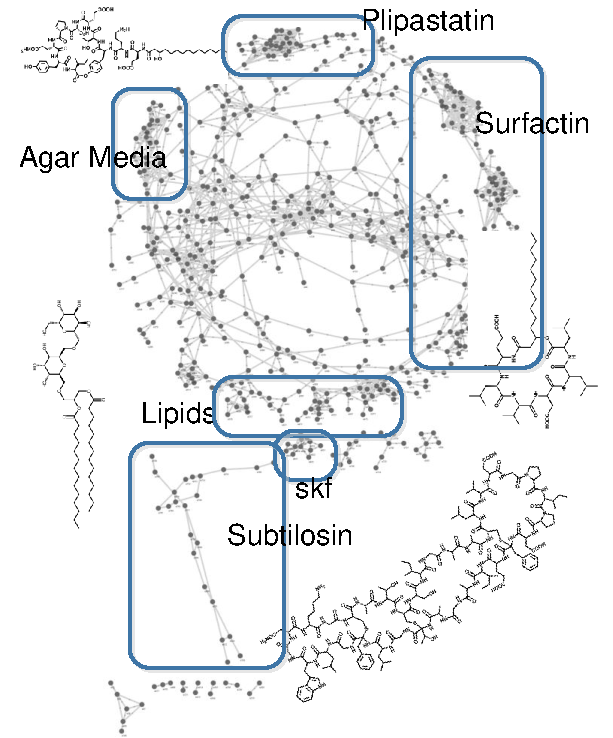
\includegraphics[height=10cm]{figures/figMolSpecNets.pdf}}

  \caption{\footnotesize{\bf Molecular spectral network of a partial {\em Bacillus subtilis} secretome.} Nodes indicate MS/MS spectra of initially-unknown compounds of any class of molecules (no peptide-specific assumptions were made), and edges indicate significant similarity between the MS/MS fragmentation patterns of different spectra, mostly between intermediates/variants of the same compounds. Selected molecular structures are shown in black overlaid with the network and next to the correspondingly highlighted network clusters.}
  \label{trd.snets.figMolSpecNets}
\end{figure}

As with peptide-based spectral networks, molecular spectral networks~\cite{watrous12} start with raw MS/MS data acquired from one or more microbial species, irrespective of the number of spectra or mass spectrometry runs. Then, similarly to the spectral alignment algorithm illustrated in \mbox{Figure~\ref{trd.snets.fig.spectralNetworks}a}, pairs of MS/MS spectra from related molecules are detected using {\em structure-independent} spectral alignment to find spectra with significantly-similar fragmentation patterns, regardless of whether the spectra are identified or not. We consider two molecules to be related if one can differs from the other by the addition, removal or replacement of a chemical group. In the special case of peptides this includes modified/unmodified versions of the same peptide, sequence polymorphisms or N/C-term sequence extensions. By avoiding peptide-specific fragmentation models and assumptions (e.g., minimum of 57~Da between matched ions in the same ion series), structure-independent spectral alignment reveals molecular networks containing not only spectra of peptides but also of primary and secondary metabolites, non-linear natural-products, lipids, glycans, and other classes of molecules. Figure~\ref{trd.snets.figMolSpecNets} shows a molecular spectral network for {\em Bacillus subtilis} %3610
and the chemical structures for several compounds corresponding to specific highlighted subcomponents of the whole network.

In brief, structure-independent spectral alignment between two spectra $x$ and $y$ solves a bipartite-matching problem between $x$ and $y$ where one part of the graph corresponds to peaks in $x$ and the other part corresponds to peaks in $y$. Nodes are connected by weighted edges if the peak masses are within mass tolerance $\delta$ of one another, (i.e., $\{|mass(p')-mass(p)|\leq\delta : p\in x, p'\in y\}$), or if the peak masses differ by $\Delta=mass(y)-mass(x)$ (i.e., $\{|mass(p')-mass(p) - \Delta|\leq\delta : p\in x, p'\in y\}$). All spectra are normalized to Euclidian norm 1 and bipartite edge weights are set to the product of intensities of the corresponding peaks with matching masses so the resulting match score is essentially an ``alignment-corrected'' generalization of a cosine between two vectors, where the standard cosine results from setting $\Delta$ to zero.
%
Once all spectrum-spectrum match scores are computed, the significantly-matched spectrum pairs are reported as a molecular spectral network where each spectrum is allowed to connect to its top $K$ scoring matches (we typically set $K$=10) and edges between spectra are retained only if in the top $K$ for both paired spectra and the match score is above the user defined threshold (usually set to 0.5-0.7, depending on sample complexity).
%This data is then imported into the free visualization program, Cytoscape, to generate display the networks. Cytoscape then produces a visual representation of the molecular network where each node (circle) represents a single discrete massconsensus spectrum and the distance between connecting nodes being indicative of the score for that estimated similarity with higher scoring matches resulting in thicker blue edges and usually in closer distances.  Depending on Cytoscape's non-deterministic network rendering algorithms, Tthis distance also depends on the direction and number of connections.

%\NeedRevision{Watrous'12: Construction of molecular spectral networks}
%
%The creation of networks using freeware such as Cytoscape (www.cytoscape.org) is often used for the global display of large data sets such as protein interactions, biochemical pathways, population networks,  and even airplane travel and their connections.ref In biology, such networks enable the direct observation of similarities as well as differences between two or more conditions where similar entities within the network are clustered together while disparate or unique entities are grouped separately. As mass spectral fragmentation of each individual molecules results in a unique MS/MS spectrum, we decided to develop networking network-based workflows to organize large data sets of tandem mass spectra based on how the similarity between fragmentation patterns of different but related precursor ions. Using a variation of Spectral Networks designed for proteomic applications, the data is initially simplified by forming consensus spectra where identical spectra exhibiting identical precursor ion mass-to-charge ratios (m/z) and fragmentation patterns are merged (Figure 2a). The simplified MS/MS data are then used for generation of the molecular networks analysis (Figure 2a). Using the same software, the spectra are then subjected to a quadratic enhancement to increase the ability to observe low mass-to-charge (m/z) ions and to lower the dominating effect that abundant ions have when comparing spectra. Vector similarities are calculated between every possible pair of spectra with a minimum of six matching ions (peaks) and similarity is determined using a modified cosine calculation that takes in account the relative intensities of the fragment ions and the precursor m/z difference between the paired spectra. This is similar toextends the concept of spectral alignment as applied in proteomics with the exception significant difference that certain peptide-specific parameters, such as the maximum difference in parent masses between two spectrautilization of peak likelihood scores replaced here with direct cosine calculations, are relaxed generalized in order to apply this approach to all classes of molecules including lipids, polysaccharides, peptides, metabolites and proteins. This is important as it is not known ahead of time what class of molecules will be ionized during analysis. Once this is completed, the significantly-matched spectrum pairs are reported as a molecular network using Matlab scripts (version) where each spectrum is allowed to connect to its top K scoring matches (we typically set K=10) and edges between spectra are retained only if in the top K for both paired spectra and the vector similarity score, represented as a cosine value, of the match is above the user defined threshold. Threshold values are usually set to 0.5-0.7 where 1.0 indicates identical spectra. This data is then imported into the free visualization program, Cytoscape, to generate display the networks. Cytoscape then produces a visual representation of the molecular network where each node (circle) represents a single discrete massconsensus spectrum and the distance between connecting nodes being indicative of the score for that estimated similarity with higher scoring matches resulting in thicker blue edges and usually in closer distances.  Depending on Cytoscape's non-deterministic network rendering algorithms, Tthis distance also depends on the direction and number of connections.
%
%Tandem mass spectra were clustered with MS-Cluster (Frank et al 2008) to group repeated acquisition of spectra from the same molecules into cluster-consensus spectra with higher signal to noise ratio; the following non-default settings were used: clustering model LTQ\_TRYP, minimum spectrum quality 0 (to avoid peptide-specific spectrum quality metrics), disabled assign-charges and correct-pm. Cluster-consensus spectra were processed by applying square root transforms to fragment peak intensities (to increase/decrease the influence of low/high intensity peaks, respectively), scaled to Euclidian norm 1 and used for the construction of molecular spectral networks in two steps: 1) pairwise spectral alignment to find pairs of spectra from related molecules and 2) selection of significant pairwise alignments to define the spectral network. For each pair of spectra S and S', spectral alignment was computed by defining modification mass M=PM(S')-PM(S) as the difference between their precursor masses and by finding matching fragment peaks between S and S' as follows: i) peaks p S and p' S' are eligible matches if |mz(p)-mz(p')|?t or if |mz(p)+M-mz(p')|?t, for a predetermined fragment m/z tolerance t; ii) match scores between matching peaks are defined as the product of their normalized peak intensities; iii) peak matches define a Bipartite Matching problem of selecting the highest scoring subset of matching peaks where each peak is matched to at most one peak in the other spectrum (a classical computer science problem with well known algorithms for finding optimal solutions). As a result of the spectrum intensity scaling and peak match scores, the optimal solution of each bipartite matching problem corresponds to the highest-possible cosine between the intensities of matched peaks (Stein et al 1994). Pairs of cluster-consensus spectra were considered for spectral alignment if their molecular masses differed by less than 45% and up to 400Da. Each spectrum retained only up to 10 highest-cosine alignments and pairwise alignments with cosine?0.7 and ?6 matched peaks were used to define spectral networks (Bandeira et al 2007) where each node is a cluster-consensus spectrum and each edge corresponds to a significant pairwise alignment. All algorithms assumed precursor mass tolerance of 1.0 Da and fragment mass tolerance of 0.3 Da.
%

%-------------------------------------------------------------------------------------
\subsubsection{Improving specificity of spectral pairs}\label{trd.snets.aim.molnets.edges}
%-------------------------------------------------------------------------------------

%
%When taken together, the set of spectra pairs defines a
%\emph{spectral network} where nodes are spectra and connections are
%defined by significant spectral alignments.

An ideal molecular spectral network for propagation of identifications would have connected spectra of related molecules and disconnected spectra from unrelated molecules.
% Decision of which connection (pair) is correct and which is incorrect should be taken with caution. In the Bandeira et al., 2007~\cite{bandeira07pnas} it is suggested to make a decision based on correlation score between two spectra.
In the current version of spectral networks~\cite{bandeira07pnas}, edges are weighted by a \emph{correlation score} calculated as a function of the percentage of the intensity in peaks matched by spectral alignment (similar to a cosine score). While this approach is discriminative enough for small datasets, it doesn't scale well to selecting significant overlaps between hundreds of thousands of different molecules, as CCMS is guaranteed to encounter in the proposed MassIVE world-wide repository for mass spectrometry data (see TRD8 for details).

While the previous aims considered either peptide-specific (aims 1-3) or instrument-tailored (SLGF, aim 2) methods to increase the accuracy of spectral networks edges determined using spectral alignment, here we propose a graph-based approach to increase the accuracy of edge scores in distinguishing correct/incorrect matches between related/unrelated molecules.
%, we propose to build on correlation scoring by taking into account neighbors of the paired spectra in the spectral network. % Intuitively, if two connected spectra come from related molecules then with high probability their neighbors should also be related and should also match.
We propose a new \emph{topological score} based on the intuition that if an edge between two spectra $x$ and $y$ is correct (i.e., their molecules are related) then $x$ should also match some or most of the neighbors of $y$. Intuitively, a larger fraction of overlapping neighbors should indicate a stronger connection between $x$ and $y$. However, there are cases when spectra may not have direct connections to the neighbors of their neighbors (i.e., spectral alignment did not detect an overlap). As exemplified in Figure~\ref{trd.snets.fig.neib_correlation}a for the pair (B,C), node C is directly connected to D but is not connected to A (A and D are neighbors of B). In this case we define the \emph{projected correlation score} between (A,C) to be equal to correlation score computed on the set of peaks from the intersection of two sets - the set of matching peaks between (A,B) (i.e., peaks of A aligned by spectral alignment to peaks of B) and the set of matching peaks between (B,C) (Figure~\ref{trd.snets.fig.neib_correlation}b). For each spectral pair $(x,y)$, the topological score is computed as an average of the correlation scores and projected correlation scores between: $i)$ $x$ and $y$, $ii)$ $x$ and the neighbors of $y$, and $iii)$ $y$ and the neighbors of $x$.

\begin{figure}[!htb]
\scalebox{1.0}{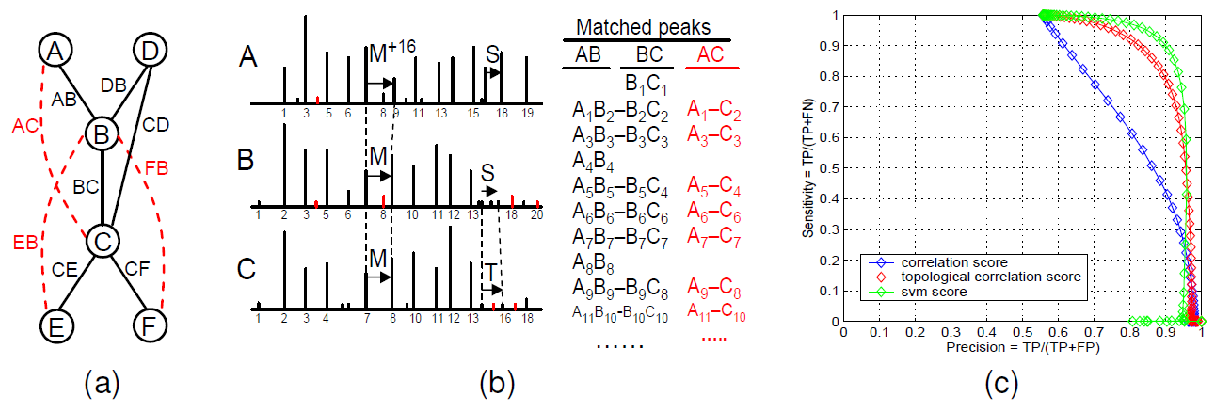
\includegraphics[width=\textwidth]{figures/figTopological.pdf}}

%\epsfxsize=5 in \centerline{
%\begin{tabular}{ccc}
%{\epsfxsize=0.9 in \epsfysize=1.6 in \epsfbox{figures/fig2a.eps} }
%&{\epsfxsize=2.5 in \epsfysize=1.7 in \epsfbox{figures/fig2b.eps} }
%& {\epsfxsize=2.0 in \epsfysize=1.7 in
%\epsfbox{figures/fig2c.eps}}\\
%(a) & (b) & (c)
%\end{tabular} }

\caption{\footnotesize{\bf Improving selection of spectral pairs via projected correlation and SVM~\cite{vapnik95} scores.} a) The topological score between B and C is computed by averaging all correlation scores (black solid line) and projected correlations (red-dashed lines). %of spectral pairs.
%
b) Example peaks matched between spectra A,B,C (VHILNVM[+16]DQAIGSHR, VHILNVMDQAIGSHR, VHILNVMDQAIGTHR). Peak indices are shown on each spectrum's x-axis and used as subscripts in the matched peaks table.
%
c) Preliminary Precision ($\frac{TP}{TP+FP}$) / Recall ($\frac{TP}{TP+FN}$) curves showing performance of classification of spectral pairs using correlation score, topological score, and SVM score. As expected, topological scores yield better separation of correct/incorrect pairs by incorporating information from each spectrum's neighborhood and the SVM classifier further improves these results by incorporating spectrum-specific probabilities of random alignment.}
\label{trd.snets.fig.neib_correlation}
\end{figure}

Preliminary precision/recall curves indicate that topological scores improve over correlation scores in distinguishing correct/incorrect spectral network edges (Figure~\ref{trd.snets.fig.neib_correlation}c). To further improve the specificity of spectral pairs we trained a Support Vector Machine%\footnote{The SVM used radial basis kernels with parameter gamma equal to 5. These settings showed the best classification performance on the training dataset.}
(SVM)~\cite{vapnik95} based on four attributes from each pair of spectra: $(i)$ correlation score, $(ii)$ topological score, $(iii)$ the p-value of the correlation score according to correlation scores between the first spectrum and its possible neighbors~\cite{bandeira07pnas}, and $(iv)$ the p-value of the correlation score computed for the second spectrum. Figure~\ref{trd.snets.fig.neib_correlation}c shows the performance of these three scoring functions among which SVM score has the best performance. We expect that the performance of topological correlation and SVM scores will improve even further as we consider different SVM kernels and provide additional input features (e.g., SLGF probabilities) to the proposed SVM model.

%-------------------------------------------------------------------------------------
\subsubsection{Improving construction of molecular spectral networks}\label{trd.snets.aim.molnets.nets}
%-------------------------------------------------------------------------------------

Spectral networks resulting from experimental data usually contain {\em true} subnetworks formed by spectra connected by correct edges (between related molecules) and {\em chimeric} networks connecting true subnetworks via a few random incorrect edges.
% As was stated before, an ideal spectral network for propagation of annotations would have connected spectra of overlapping peptides and disconnected spectra of non-overlapping peptides. The \emph{true networks} are formed by spectra connected via true spectral pairs. A \emph{mixed networks} is a mixture of true networks connected by false spectral pairs.
Note that just one incorrect edge suffices to connect two true networks into a single chimeric network, regardless of the number of correct edges in the true subnetworks. In difference from aim 2, where we propose a peptide-specific approach (using network dictionaries) to define connected components in spectral networks, here we propose a structure-independent graph-based algorithm for molecular spectral networks based on a well known clustering algorithm.
% Since annotations in spectral networks are propagated across the connections it is crucial for spectra of overlapping peptides to be in the same network, and spectra of different peptides to be in different networks.

A simple way to split chimeric networks into true subnetworks is to threshold edge scores: pairs with SVM score above a given threshold are considered true and otherwise rejected as false; the threshold would be chosen based on the precision/recall curves from Figure~\ref{trd.snets.fig.neib_correlation}c. While this procedure performs well for removing false spectral pairs, the quality of removing false connections between true subnetworks can still be further improved. The key observation is that for a spectral pair $(x,y)$ the SVM score is computed {\em statically} based on the correlation score between $x$, $y$ and their neighbors. In particular, it does not consider how the scores could change by {\em iteratively} adding (presumably correct) or removing (presumably incorrect) neighbor spectra to the two subnetworks connected by $(x,y)$.
%
%Considering would target some cases when a pair classified as true is the only one (or a part of few) connections between different true networks. Intuitively, this pair is not classified correctly, therefore; an additional support is required and is obtained by grouping spectra into putative networks and removing pairs which connect two putative networks.

\begin{table}[!h]
 {\footnotesize
\begin{center}
\begin{tabular}{@{}crrrr@{}}
\cline {2-5} {}&   \multicolumn{4} {c} {}\\[-2ex]
 {Number of true subnetworks}     & \multicolumn{2} {c} {NetWeaver} & \multicolumn{2} {c}{SVM}  \\
 {per spectral network}     &  {\# networks} & {\# spectra} &  {\# networks} & {\# spectra}\\
\hline
 {\scriptsize singleton} &  80345 & 80345 & 75369 & 75369  \\
 $1$ & 11086  & 41270 & 9385 & 41606  \\
 $2$ & 749  & 2823 & 708 & 4793  \\
 $3$ & 109  & 476 & 113 & 1133  \\
 $4$ & 28  & 173 & 34 & 325 \\
 $5$ & 9  & 45 & 13 & 303 \\
 $6$ & 1  & 6 & 4 & 41 \\
 $7$ & 0  & 0 & 3 & 88 \\
 $8$ & 0  & 0 & 2 & 31 \\
 $9$ & 0  & 0 & 1 & 13 \\
 $10$ & 0  & 0 & 4 & 118 \\
 ~~$11^{+}$ & 1  & 99 & 7 & 1253  \\
\hline
  \multicolumn{2} {l} {\textbf{Mixing accuracy}} &   \multicolumn{1} {r} {\textbf{0.990}} &\multicolumn{2} {r} {\textbf{0.958}}\\
\end{tabular}
\end{center} }
\caption{\footnotesize{\bf Mixing statistics of spectral networks before and after applying the proposed NetWeaver algorithm.} Mixing is measured by the number of true subnetworks in a spectral network (left column). A perfect algorithm would separate all cases with 2 or more true networks (chimeric networks) into networks with only 1 true subnetwork while avoiding splitting true networks into singletons or multiple networks;
%; Splitting indicates the number of true clusters
%(and number of spectra) which contain %overlap with
%$k$ putative clusters;
\emph{singletons} are networks of size one (isolated non-paired spectra).
%$11^{+}$ - number of overlapping clusters is higher or equal to eleven.
Mixing accuracy represents the average ratio of correctly grouped spectra by the total number of grouped spectra (over all putative networks). \label{cast_perform}}
\end{table}

%The putative networks are gathered by a clustering method based on pairwise similarity $similarity(x,y)$ between spectra which is equal to SVM score for $(x,y)$.
We propose a new neighbor-based clustering algorithm \emph{NetWeaver} to combine spectral pairs into spectral networks. NetWeaver adds or removes an element from the network based on similarity with neighbors already in the network. This is different from classical clustering approaches where similarity is computed to {\em all} elements in the cluster. This is because we aim to group not only repeated spectra from the exact same molecule, but also spectra from related but distinct molecules. Inspired by the CAST~\cite{bendor99} clustering algorithm for analysis of gene expression, we iteratively check for elements to be added or excluded from the network. The main difference is in the definition of the similarity function between an element and a cluster. In CAST the similarity between an element $x$ and a cluster $C$ is defined as $similarity(x,C)=\sum_{y \in C}{similarity(x,y)}/|C|$. In contrast, in NetWeaver the similarity is defined as $similarity(x,C)=\sum_{y \in N(x)\cap
C}{similarity(x,y)}/|N(x)\cap C|$, where $N(x)$ is the set of neighbors of $x$, e.g., spectra connected to spectrum $x$ by spectral pairs. The algorithm starts with a cluster of size one, and iteratively applies the following rules: \emph{(i)} an element $x \in S$ (set of non-clustered elements) is added to $C$ if $similarity(x,C) = max_{y\in S}\{similarity(y,C)\}$ and $similarity(x,C)$ is above a given threshold $T^+$, \emph{(ii)} an element $x \in C$ is removed from $C$ if $similarity(x,C\setminus\{x\}) =
min_{y\in C}\{similarity(y,C\setminus\{y\})\}$ and $similarity(x,C\setminus\{x\})$ is bellow a given threshold $T^-$. If after applying both rules the network does not change then we proceed to another subnetwork.
%
%In Table \ref{cast_perform} we evaluate the quality of spectral networks before and after clustering.
\emph{Putative} networks are formed by either retaining all spectral pairs classified as true according to thresholded SVM scores (SVM) or as networks constructed with the proposed clustering algorithm (NetWeaver).
%The primary goal is to have less putative networks which mix more than one true network. That would imply that number of false spectral pairs is reduced.
As shown in Table~\ref{cast_perform} using a dataset of annotated peptide spectra, preliminary results indicate that NetWeaver substantially reduces the number of putative spectral networks with more than one true subnetwork.

%The small increase in the number of true clusters which split into
%more than one putative clusters may slightly reduce the number of
%propagated annotations. Notice that it is more important to avoid
%incorrect identifications caused by excessive mixing than to miss
%some identifications because of excessive splitting.

%Our dataset contains peptides with mutations and modifications whose spectra should be allowed to be clustered together with their unmodified versions. Therefore, when computing the numbers for mixing (see Table \ref{cast_perform}) we relax the definition of true spectral pair -- the overlap between two peptides is true if they are prefix/suffix peptides with less or equal to 5 amino acids difference in length, and up to 2 mutations.
%%However, if mutated/modified versions of a peptide fall into
%%different putative clusters it should not be counted as a splitting
%%error, because in fact the peptides are different. Therefore, when
%%computing the numbers for splitting (see Table \ref{cast_perform})
%%the definition of a true pair is more stringent -- the overlap
%%between two peptides is true if they are prefix/suffix peptides with
%%less or equal to 2 amino acids difference in length, and 0
%%mutations.
%To avoid distortion of the numbers presented in Table~\ref{cast_perform} by small insignificant networks when reporting
%splitting of true networks by putative networks we count the number of true networks with largest overlap with a putative networks and the set of counted networks should overlap with at least 95\% of the putative networks.

%Similarly, for the mixing of true components by putative components
%we count putative components with largest overlap with a true
%component and the set of counted components should cover at least
%95\% of the true component.


%%**************************************************************************************
%% ------------------------------------------------------------------------------------
%\section{Summary}
%% ------------------------------------------------------------------------------------
%%**************************************************************************************

%**************************************************************************************
% ------------------------------------------------------------------------------------
\section{Driving Biomedical Projects (DBPs)}
% ------------------------------------------------------------------------------------
%**************************************************************************************

DBP1 (unraveling histone code), DBP2 (analyzing polybacterial infections), DBP3 (interspecies chemical interactions), DBP5 (therapeutic antibody development), DBP6 (molecular networks in diabetes), DBP7 (clinical cancer proteogenomics), DBP10 (analyzing cataractous lens).

% For all 3 aims

\bibliographystyle{plain}
%\bibliographystyle{snets}{unsrt}
%\bibliographystyle{snets}{ieeetr}

%\bibliography{snets}{bibfiles/nb_msms,bibfiles/bandeiraLab,bibfiles/naturalproductsVenom,bibfiles/immunology}{Literature cited}
\bibliography{../../bibtex/msms,../../bibtex/bandeiraLab,../../bibtex/naturalproductsVenom,../../bibtex/immunology}

\end{document}
